%======================================================================
% Crypto World Bank — BCOLBD 2026 Student Category White Paper
% Blockchain Track | Times New Roman 11 pt | single spacing
% Hard limit: 20 pages including cover, figures, and references
% Source content: project specification (v40); this file is standalone.
%======================================================================
\documentclass[11pt,a4paper]{article}

\usepackage{fontspec}
\setmainfont{Times New Roman}
\setsansfont{Times New Roman}

\usepackage[a4paper,top=18mm,bottom=18mm,left=18mm,right=18mm]{geometry}
\usepackage{setspace}
\setstretch{1.0}
\usepackage{microtype}
\usepackage{graphicx}
\graphicspath{{images/}}
\usepackage{xcolor}
\usepackage{booktabs}
\usepackage{array}
\usepackage{tabularx}
\usepackage{colortbl}
\usepackage{multirow}
\usepackage{enumitem}
\usepackage{caption}
\usepackage{subcaption}
\usepackage{float}
\usepackage{titlesec}
\usepackage{fancyhdr}
\usepackage{tikz}
\usepackage{amsmath,amssymb}
\usepackage{hyperref}
\newcommand{\rcite}[1]{[\ref{#1}]}
\newcommand{\rcites}[2]{[\ref{#1}, \ref{#2}]}

\definecolor{CoverNavy}{HTML}{0B1F3A}
\definecolor{CoverGold}{HTML}{C4A35A}
\definecolor{CoverInk}{HTML}{1A1A1A}
\definecolor{RowShade}{gray}{0.94}
\definecolor{HeadShade}{gray}{0.88}
\definecolor{RuleGray}{gray}{0.55}

\captionsetup{
  font={small},
  labelfont={bf},
  skip=4pt,
  justification=centering
}
\titleformat{\section}{\normalsize\bfseries\color{CoverNavy}}{\thesection.}{0.5em}{}
\titleformat{\subsection}{\normalsize\bfseries\color{CoverInk}}{\thesubsection}{0.45em}{}
\titleformat{\subsubsection}{\normalsize\itshape\color{CoverInk}}{\thesubsubsection}{0.4em}{}
\titlespacing*{\section}{0pt}{0.85em}{0.35em}
\titlespacing*{\subsection}{0pt}{0.65em}{0.25em}
\titlespacing*{\subsubsection}{0pt}{0.45em}{0.2em}

\setlist[itemize]{leftmargin=1.15em,itemsep=0.12em,topsep=0.2em,parsep=0pt}
\setlist[enumerate]{leftmargin=1.25em,itemsep=0.12em,topsep=0.2em,parsep=0pt}
\setlength{\parindent}{0pt}
\setlength{\parskip}{0.38em}
\setlength{\tabcolsep}{4pt}
\renewcommand{\arraystretch}{1.12}

\newcommand{\tablehead}{\rowcolor{HeadShade}\bfseries}
\newcommand{\Y}{\textbf{Y}}
\newcommand{\N}{\textbf{N}}
\newcommand{\Pmark}{\textbf{P}}

\pagestyle{fancy}
\fancyhf{}
\fancyhead[L]{\small\color{CoverNavy} Decentralized Crypto World Bank \textbullet\ BCOLBD 2026}
\fancyhead[R]{\small\color{CoverNavy} Student Category \textbullet\ Blockchain}
\fancyfoot[C]{\small\thepage}
\renewcommand{\headrulewidth}{0.4pt}
\renewcommand{\footrulewidth}{0pt}

\hypersetup{
  colorlinks=true,
  linkcolor=CoverNavy,
  urlcolor=CoverNavy,
  citecolor=CoverNavy,
  pdftitle={Decentralized Crypto World Bank: A Blockchain-Based Banking Platform with AI-Enhanced Security and Assistance},
  pdfauthor={Md. Bokhtiar Rahman Juboraz; Md. Mahir Ahnaf Ahmed},
  pdfsubject={BCOLBD 2026 Student Category White Paper},
  pdfkeywords={blockchain, DeFi, hierarchical lending, governance, Bangladesh}
}

\begin{document}
\thispagestyle{empty}

%----------------------------------------------------------------------
% COVER
%----------------------------------------------------------------------
\begin{tikzpicture}[remember picture,overlay]
  \fill[CoverNavy] (current page.north west) rectangle ([yshift=-38mm]current page.north east);
  \fill[CoverGold] ([yshift=-38mm]current page.north west) rectangle ([yshift=-39.6mm]current page.north east);
\end{tikzpicture}

\vspace*{-8mm}
\begin{center}
{\color{white}\large\bfseries BLOCKCHAIN OLYMPIAD BANGLADESH}\\[0.25em]
{\color{white}\normalsize BCOLBD 2026}\\[0.45em]
{\color{CoverGold}\small STUDENT CATEGORY \textbullet\ BLOCKCHAIN TRACK \textbullet\ WHITE PAPER}
\end{center}

\vspace{8mm}
\begin{center}
{\LARGE\bfseries\color{CoverNavy} Decentralized Crypto World Bank}\\[0.4em]
{\large\color{CoverInk} A Blockchain-Based Banking Platform\\[0.1em]
with AI-Enhanced Security and Assistance}
\end{center}

\vspace{2.6mm}
{\color{CoverGold}\hrule height 0.7pt}
\vspace{2.8mm}

\noindent
{\small
\begin{tabularx}{\textwidth}{@{}>{\bfseries}p{2.6cm}X>{\bfseries}p{2.2cm}p{4.4cm}@{}}
Project & Decentralized Crypto World Bank (CWB) & Category & Student \textbullet\ Blockchain \\
Team & Sparta & Team ID & \texttt{6a79873991221} \\
Type & Permissioned-role public EVM DApp & Year & 2026 \\
Network & Ethereum Sepolia (primary); Polygon Amoy (secondary) & Prototype & UI + on-chain write \\
Repository & \multicolumn{3}{X}{\url{https://github.com/Yuvraajrahman/Cryto-World-Bank}} \\
\end{tabularx}
}

\vspace{2.2mm}
\noindent\textbf{Team Sparta}
\vspace{1mm}

\noindent
{\small
\begin{tabularx}{\textwidth}{@{}>{\bfseries}p{4.7cm}p{3.3cm}X@{}}
\toprule
\tablehead Member & Role & Responsibilities \\
\midrule
Md.\ Bokhtiar Rahman Juboraz & Team Lead & Smart-contract architecture, four-tier capital design, oracle and ML risk pipeline, security model \\
Md.\ Mahir Ahnaf Ahmed & Co-author & Application layer (API, React UI, wallet flows), data partitioning, partner and go-to-market design \\
\bottomrule
\end{tabularx}
}

\vspace{3.4mm}
\noindent
\colorbox{HeadShade}{%
\begin{minipage}{\dimexpr\textwidth-2\fboxsep\relax}
\vspace{1.6mm}
\textbf{Abstract.}
Development finance is a multi-party coordination problem. Supranational reserves, national development banks, local lenders, retail borrowers, depositors, and regulators must move capital together, yet they do not trust one another enough to share a single private ledger. Correspondent banking locks idle funds in nostro/vostro accounts, cross-border payments still cost about \$45 and take two to five days, remittance corridors average 6.49\% against a 3\% SDG target, 1.4~billion adults remain unbanked, and MSMEs face a \$4.5~trillion annual financing gap. Flat DeFi pools (Aave, Compound, Maker) automate lending at scale but have no institutional hierarchy, no reserve-ratio enforcement across tiers, and no Local-Bank-to-client path that microfinance actually uses. \textit{Crypto World Bank} encodes that hierarchy on a public Proof-of-Stake EVM: Tier~1 World Bank reserve $\to$ Tier~2 National Banks $\to$ Tier~3 Local Banks $\to$ Tier~4 clients. Smart contracts enforce reserve ratios, role-based access, loan state machines, solidarity-group liability, and soulbound Credit Passports. Off-chain AI (Random Forest + Isolation Forest + SHAP; held-out F1~$=$~0.891) advises human approvers; it never auto-disburses. Partner incentives---cheaper wholesale liquidity, portable reputation, liquidator bonuses, depositor yield---are allocated on-chain, not by side letters. This white paper follows the BCOLBD Blockchain evaluation scheme: Problem \& Solution, Market \& Partners, Competition \& Risks, Architecture \& Governance, and Revenue \& Distribution.
\vspace{1.2mm}

\noindent\textbf{Keywords:} hierarchical DeFi, development finance, programmable reserves, soulbound credit, multi-party governance, oracle-mediated risk, Bangladesh sandbox
\vspace{1.4mm}
\end{minipage}%
}

\vspace{3.2mm}
{\small\noindent\textit{Document control.} English original. Format: Times New Roman 11~pt, single spacing, $\leq$20 pages including all material (BCOLBD 2026 Blockchain Guideline). Evaluation mapping: Section~1 $\to$ 30 pts; Section~2 $\to$ 10 pts; Section~3 $\to$ 20 pts; Section~4 $\to$ 30 pts; Section~5 $\to$ 10 pts.}

\clearpage
\setcounter{page}{2}

%----------------------------------------------------------------------
\section{Problem and Solution}
\label{sec:problem}
% 30 points
%----------------------------------------------------------------------

\subsection{A multi-party problem that a database cannot settle}

Global development finance is not a single-firm workflow. Capital is supposed to travel from a supranational reserve through national and local intermediaries to a shopkeeper or a solidarity group, and then back again as repayments, interest, and surplus. Each hop is a different legal person with a different incentive: the reserve wants solvency and mandate compliance; the national bank wants jurisdictional control and political cover; the local bank wants origination fees without being stuck with default; the borrower wants cheap, fast credit without surrendering identity documents to every counterparty; the regulator wants an audit trail that nobody can quietly rewrite after the fact.

Those parties already have databases. What they do not have is a \textbf{shared, tamper-evident rulebook that executes even when they disagree}. Building bilateral trust---legal opinions, correspondent accounts, quarterly audits, reconciling three ledgers after every disbursement---is the cost centre. The World Bank's own FundsChain programme and wholesale experiments such as JPMorgan Kinexys show that institutions will put \textit{logs} on a ledger. They still do not encode the \textit{rules}: minimum reserve ratios, who may allocate downward, who may freeze an account, and how a group of unbanked borrowers can share liability without a paper contract that a court in a second country must enforce.

The friction is measurable:
\begin{itemize}
  \item \textbf{Idle capital.} Correspondent banking pre-funds nostro/vostro accounts so each corridor can settle; that float cannot be lent~\rcite{cpmi147}.
  \item \textbf{Slow, expensive settlement.} Typical cross-border transfers take two to five days and cost about \$45 per payment~\rcite{fsb2020}.
  \item \textbf{Regressive remittance prices.} Average corridor charges of 6.49\% sit above the UN SDG 3\% target~\rcite{wbremit}.
  \item \textbf{Exclusion.} 1.4~billion adults are unbanked~\rcite{findex}; MSMEs face a \$4.5~trillion annual credit gap~\rcite{ifc2017}.
  \item \textbf{Opaque reserves.} Lower-tier clients cannot verify that a parent still holds the buffer it claims; audits arrive quarterly, after the damage.
  \item \textbf{Re-underwriting.} Each institution scores the same borrower from a private file. There is no portable, non-transferable credit history that a competing local bank can trust without calling the first bank's risk officer.
\end{itemize}

This is exactly the class of problem BCOLBD asks for: many parties, misaligned incentives, and a trust gap that no amount of API integration closes---because the API still has an operator who can change yesterday's balance.

\subsection{Why blockchain, not a conventional cloud}

A well-designed PostgreSQL cluster with row-level security can store loans. It cannot do four things that this problem requires:

\begin{enumerate}
  \item \textbf{No single operator of truth.} If the National Bank hosts the database, Local Banks will not accept its reserve figures in a dispute. If a vendor hosts it, every participant must trust that vendor's administrators, backups, and jurisdiction. A public EVM chain makes reserve balances, loan state, and role grants independently verifiable by any party (including a regulator with a read-only node).
  \item \textbf{Atomic multi-party state.} When a Local Bank disburses, the parent's remaining allocatable reserve, the client's Credit Passport, the installment schedule, and the insurance buffer must move together or not at all. Smart contracts give that atomicity; a cloud workflow gives eventual consistency and reconciliation tickets.
  \item \textbf{Programmable enforcement, not policy PDFs.} ``Do not allocate below a 20\% reserve ratio'' is a sentence until it is a \texttt{require()} that reverts. Hierarchy, borrowing caps, group consent, and pause switches become consensus-checked transitions, not emails.
  \item \textbf{Incentive allocation on the same rail as the asset.} Liquidator bonuses, depositor ERC-4626 shares, interbank pool interest, and protocol spreads are paid by the contract that holds the funds. Side letters cannot silently divert them.
\end{enumerate}

Flat public DeFi already proves that lending can run without a licensed custodian (Aave~v3 about \$26.3B TVL; broader DeFi lending above \$55B~\rcites{defillama}{aavev3}). It does \textit{not} prove that development-bank \textit{organisation} can. Those protocols are one pool, many assets, token-weighted governance. They have no World~$\to$National~$\to$Local~$\to$Client mandate, no solidarity group with mutual liability, and no human credit officer in the loop for under-collateralised MSME loans. Institutional DeFi (Maple, Goldfinch) serves accredited lenders, not a four-tier public-development stack~\rcites{werner2022}{maple}.

CWB's claim is therefore narrow and falsifiable: \textbf{blockchain is the only practical way to let mutually distrusting financial institutions share capital rules in real time, while still letting a local officer say yes or no to a human borrower.}

\begin{figure}[H]
\centering
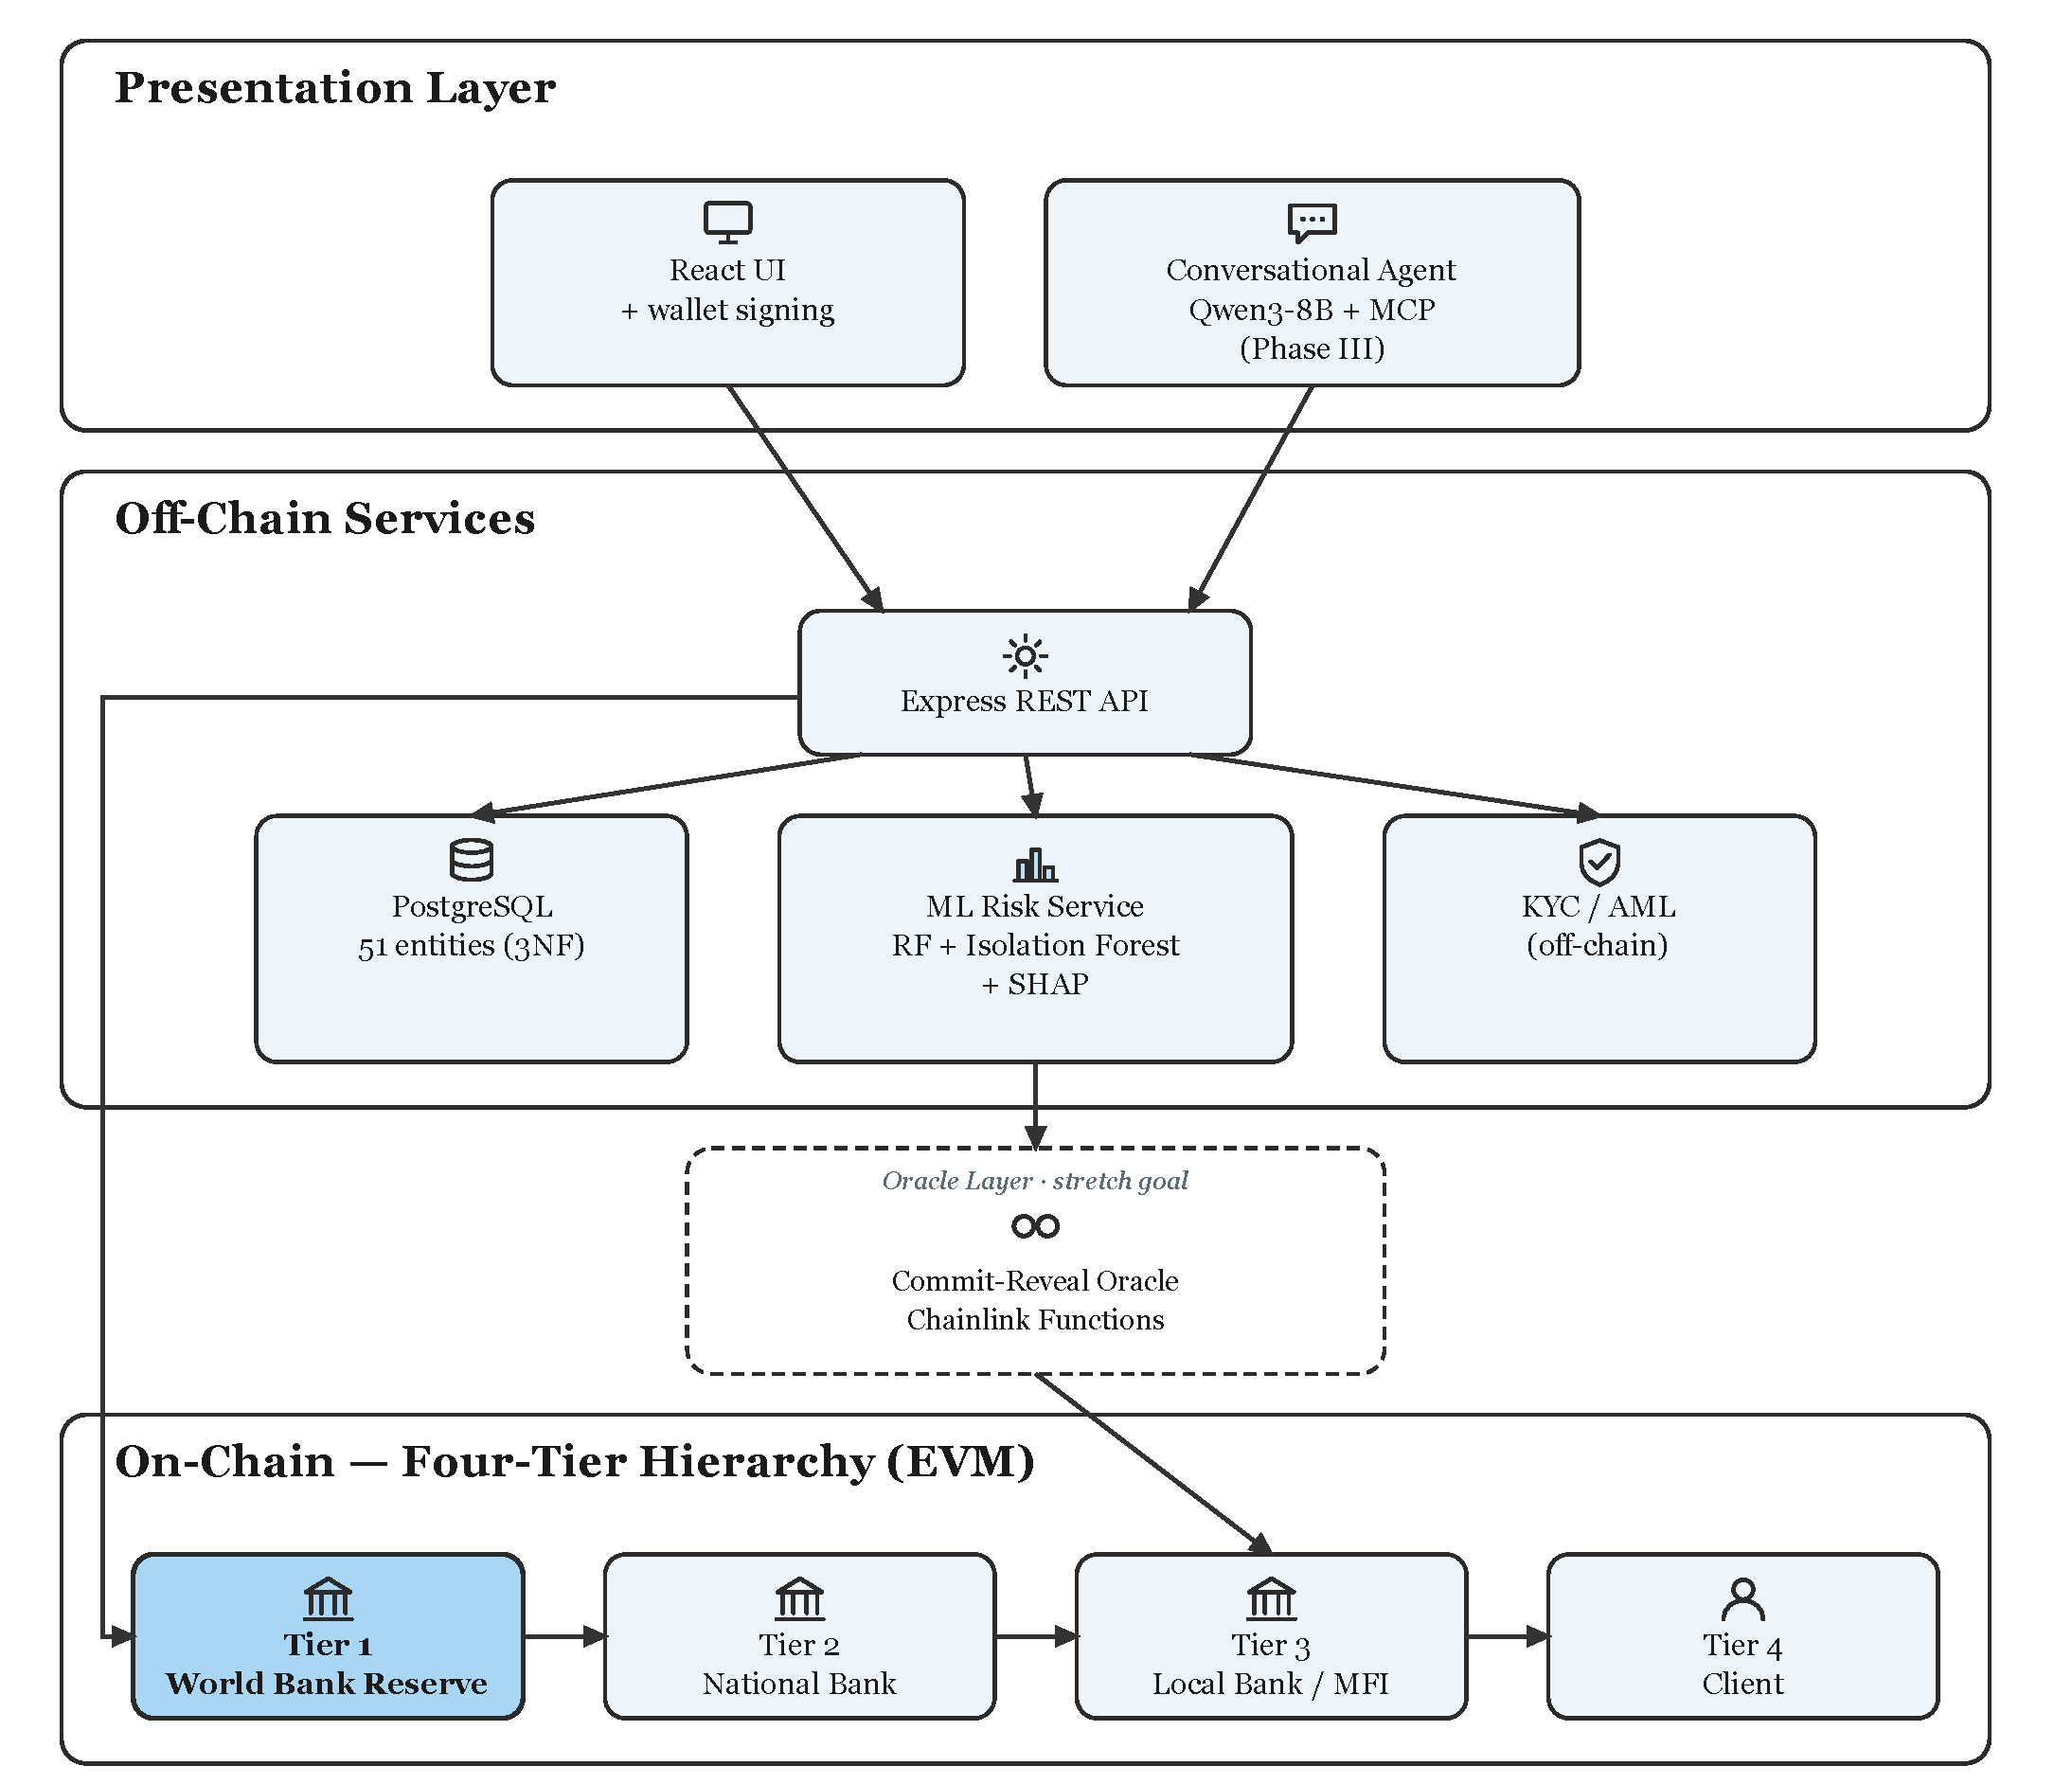
\includegraphics[width=0.64\textwidth,keepaspectratio]{architecture_diagram_fixed.pdf}
\caption{System overview: four-tier on-chain banks, off-chain services, and human-gated AI.}
\label{fig:overview}
\end{figure}

\subsection{The solution: a hierarchical on-chain development bank}

CWB implements six classical banking functions as contracts rather than as discretionary operations: deposit mobilisation, credit allocation, payment and settlement, risk intermediation, liquidity management, and ancillary services (FX, insurance buffer). Participants fall into three categories: a programmable Tier~1 reserve, licensed Tier~2/3 institutions, and Tier~4 retail (individuals and solidarity groups of 3--20 members).

Capital does not only flow downward. Banks borrow from same-tier peers (\texttt{InterBankLendingPool}), park surplus with a parent (\texttt{UpwardDepositFacility}), and co-fund large loans (\texttt{SyndicatedLoan}). Retail products include collateralised and credit-based loans, ERC-4626 savings, installment repayment, and a non-transferable Credit Passport (soulbound token) that stores score, tier, and repayment history---not name, NID, or selfie.

\begin{figure}[H]
\centering
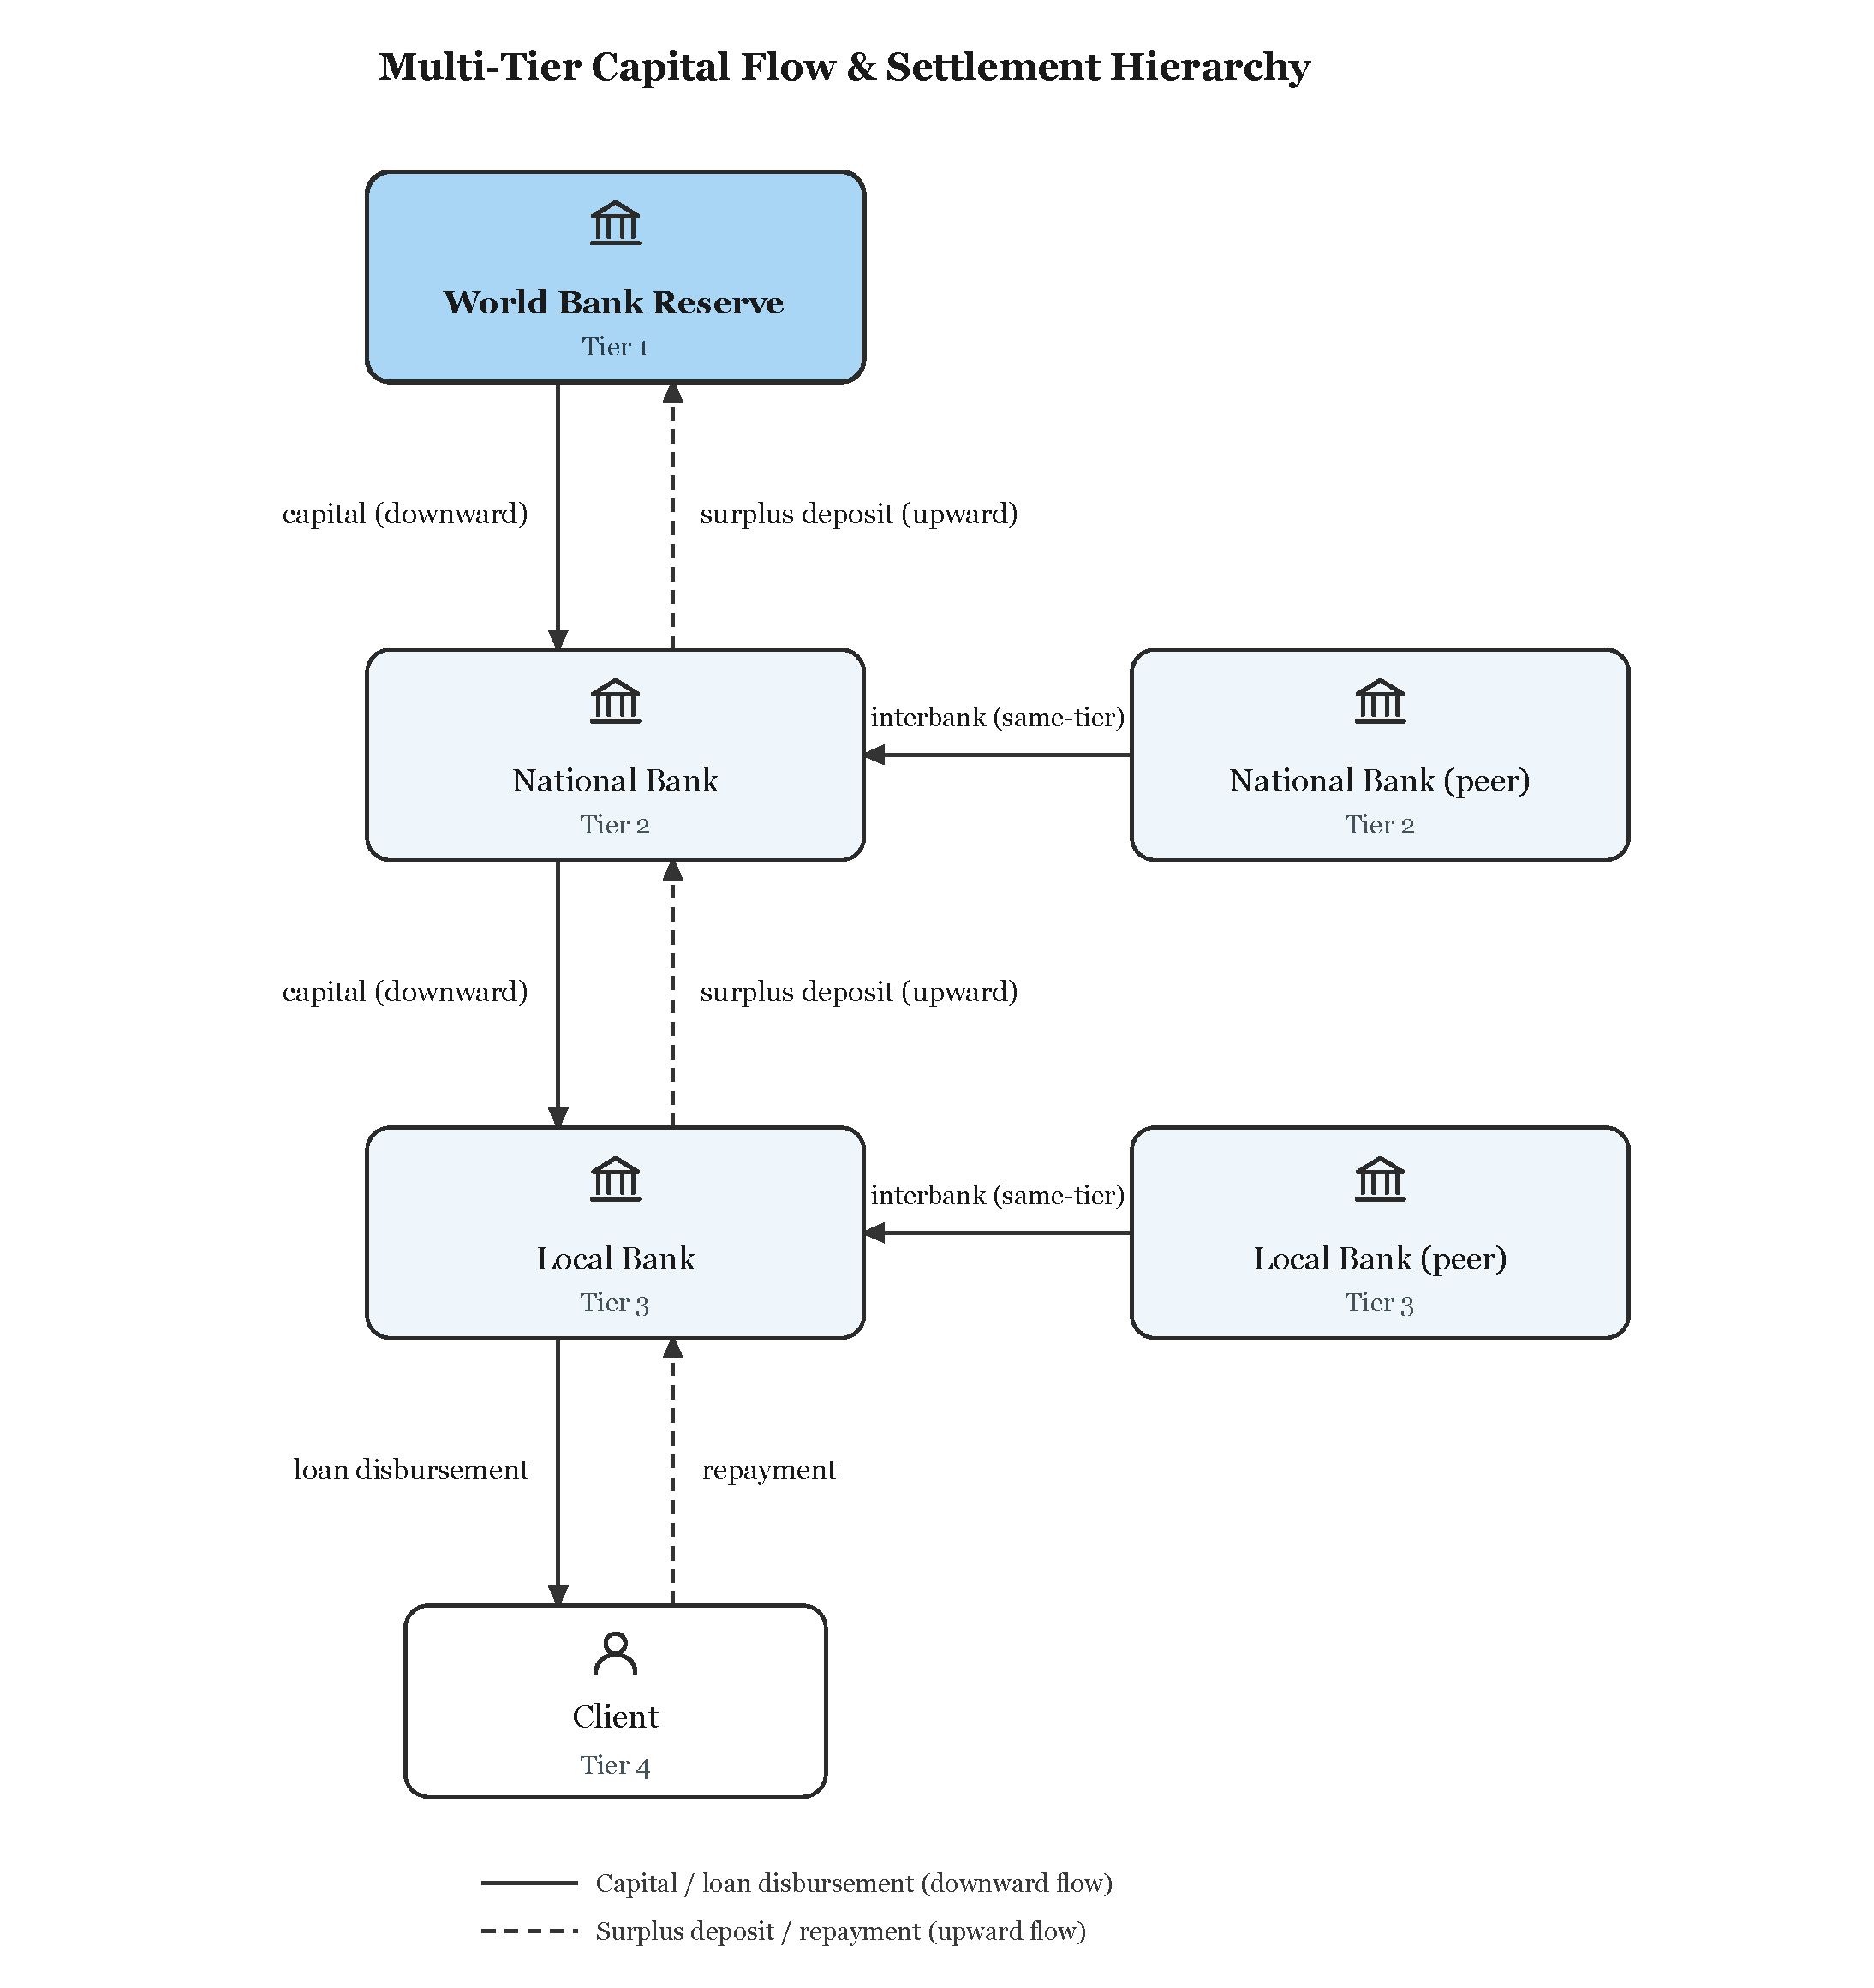
\includegraphics[width=0.62\textwidth,keepaspectratio]{fund_flow_diagram_v2.pdf}
\caption{Cross-tier and same-tier capital flows that a flat pool cannot express.}
\label{fig:flows}
\end{figure}

\textbf{Loan lifecycle (authoritative on-chain).} Request $\to$ off-chain ML score commit--reveal $\to$ Local Bank approver decision $\to$ disbursement $\to$ installment schedule $\to$ repayment or health-factor path. The ML service (Random Forest fraud probability, Isolation Forest anomaly, stacking meta-score, SHAP explanation) writes a hash $h=\mathrm{keccak256}(s\|\mathrm{nonce})$ before reveal, so the score cannot be edited after the officer has seen it. Combined score $s<0.4$ suggests approve, $0.4\le s<0.7$ forces manual review, $s\ge 0.7$ suggests reject. \textbf{No contract auto-disburses from a model output.} That is a product decision, not a limitation: unsecured and thinly collateralised development credit is a regulated judgment, and EU-style explainability (Art.~86 spirit) plus a human gate is how the system stays deployable.

\textbf{Stablecoin-first unit of account.} Retail users are not asked to hold volatile ETH as working capital. Pools are denominated in USD-stable value (\texttt{MockUSDC} on testnet; authorised stablecoins in a sandbox). This matches MiCA / GENIUS-style treatment of fiat-referenced tokens and keeps loan math intelligible to a local credit officer.

\textbf{What is in scope for the competition prototype.} Four-tier contracts, RBAC, loan state machine, reserve checks, React + wallet UI that writes to chain, Express API, FastAPI ML scoring (F1~$=$~0.891 on a 5{,}140-row held-out wallet-grouped split of BCCC-DeFiFraudTrans-2025), and an optional MCP conversational agent that can read state and propose writes only after explicit confirmation. Mainnet, live KYC vendors, and production Chainlink DON are design upgrades, not claimed as finished.

\begin{figure}[H]
\centering
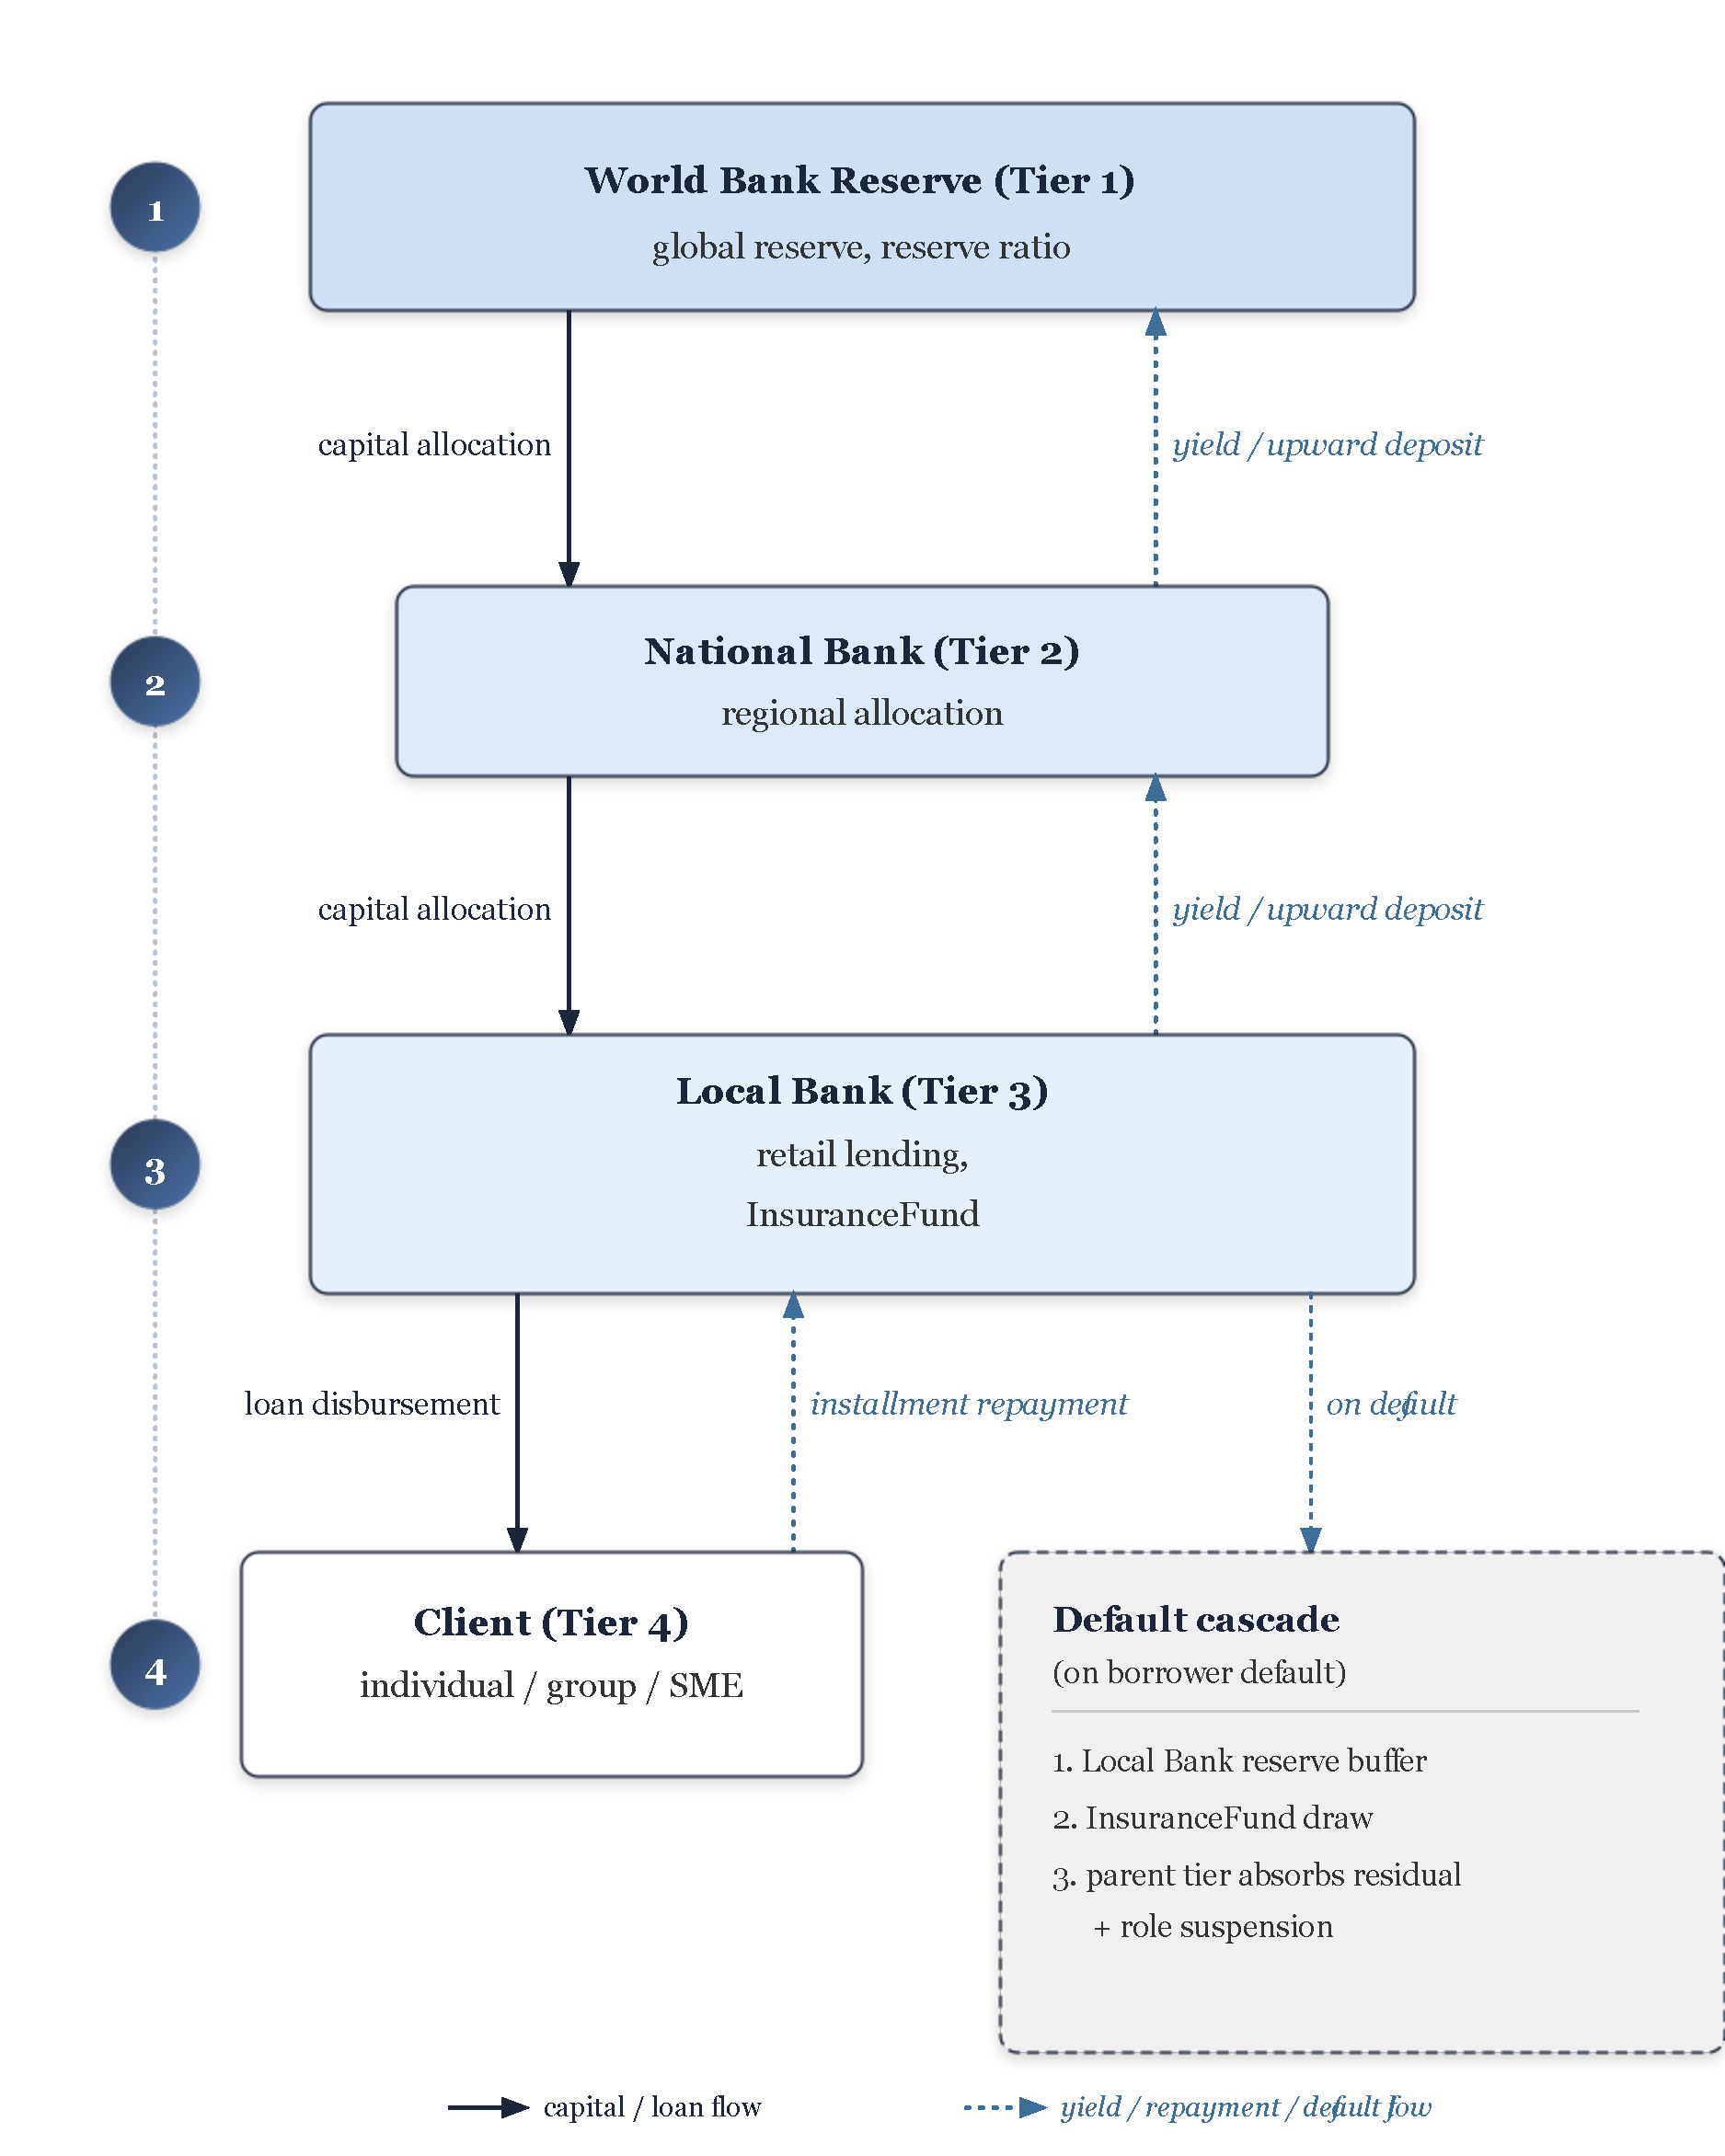
\includegraphics[width=0.60\textwidth,keepaspectratio]{fig-hierarchical-banking.pdf}
\caption{Four-tier capital: downward allocation and upward repayment on the same ledger.}
\label{fig:fourtier}
\end{figure}

%----------------------------------------------------------------------
\section{Market and Partners}
\label{sec:market}
% 10 points
%----------------------------------------------------------------------

\subsection{Market definition}

CWB is not ``another Aave for Bangladesh.'' It is infrastructure for \textbf{supervised hierarchical credit} in markets where correspondent banking is expensive and MSME files do not travel. We segment as follows.

\textbf{TAM (global development-finance and MSME credit gap).} The IFC MSME gap of \$4.5~trillion per year is the ceiling of unmet credit CWB-style rails could eventually touch~\rcite{ifc2017}. DeFi lending TVL (tens of billions) shows that on-chain origination already clears, but it currently serves crypto-native collateral, not local-bank clients~\rcite{defillama}.

\textbf{SAM (South Asia + corridor finance).} Bangladesh is the design beachhead: large inward remittances, dense mobile-financial-service (MFS) cash-in/out, a mature microfinance culture (group liability), and a regulator that has already experimented with digital-bank and sandbox instruments. Adjacent demand exists wherever national development banks on-lend World Bank / IDA-style lines and cannot show live reserve compliance to the next tier.

\textbf{SOM (sandbox, 36 months).} One licensed local lender (or a development-bank innovation unit) + 300--1{,}000 retail/MSME wallets on a permissioned-role deployment. Revenue math in Section~\ref{sec:revenue} is built on this SOM, not on TAM slogans: break-even on the order of 200--300 active loans at a \$25{,}000 average ticket under the stated default and gas assumptions.

Primary customer is the \textbf{Local Bank} (Tier~3): it originates, collects documents, and signs. National Banks buy \textbf{allocatable liquidity with on-chain proof of downstream use}. Retail clients are users, not the first sales call---except solidarity groups that a partner MFI already organises.

\subsection{Partners that the solution cannot work without}

\begin{table}[H]
\centering
\small
\caption{Ecosystem partners, value added, and on-chain incentive.}
\label{tab:partners}
\begin{tabular}{@{}>{\raggedright\arraybackslash}p{3.2cm}>{\raggedright\arraybackslash}p{4.6cm}>{\raggedright\arraybackslash}p{6.0cm}@{}}
\toprule
\tablehead Partner & Why the system needs them & Incentive allocated on-chain \\
\midrule
National / development banks (Tier~2) & Legal corridor into the jurisdiction; wholesale capital & Cheaper interbank rate $r_{\mathrm{IB}}(U)\le r_{\mathrm{down}}(U)-\delta$; live reserve attestation \\
\rowcolor{RowShade}
Local banks / MFI branches (Tier~3) & Last-mile origination, cash handling, human approval & Origination inside the fee split; portable Credit Passport reduces repeat KYC cost \\
MFS / payment gateways (cash-in/out) & Fiat on-ramp for unbanked clients who will not hold gas tokens & Corridor volume; optional FXModule spread when a dual-currency hop is used \\
\rowcolor{RowShade}
KYC/AML vendors \& NID rails & Level~1/2 identity without putting PII on-chain & Paid off-chain; only document hashes and role flags hit the ledger \\
Regulators (sandbox / supervisor node) & Licence to operate credit; SAR/freeze legitimacy & Read-only event access; cannot be locked out of the audit log by a bank admin \\
\rowcolor{RowShade}
Oracle \& automation (Chainlink path) & Prices, Proof of Reserve, overdue upkeep & Protocol fee on FX and attested reserve queries (production upgrade) \\
Independent liquidators & Close $HF<1$ positions without a central workout desk & 5--8\% bonus paid by \texttt{LiquidationEngine} \\
\rowcolor{RowShade}
Depositors (ERC-4626) & Local stablecoin liquidity & Vault yield; withdrawals gated by the same reserve ratio as loans \\
Open-source builders & Contract review, regional localisation & No token grant in the prototype; reputation and fork rights \\
\bottomrule
\end{tabular}
\end{table}

Partner incentives are not a memorandum of understanding. A Local Bank that keeps a healthy reserve can lend onward; if it breaches the ratio, \texttt{allocateCapital} reverts---the parent does not need to ``choose'' to punish it. A depositor earns because \texttt{SavingsVault} splits interest among depositor yield, \texttt{InsuranceFund} (5\% capture for default cover), and protocol revenue. A group member's consent is a contract signature, not a field officer's notebook.

\textbf{Bangladesh-shaped collaboration.} MFS operators are complementary last-mile cash, not competitors to the ledger. Group lending is the on-chain analogue of existing solidarity practice (3--20 members, mutual liability, per-member share), without claiming to replace social enforcement. The first regulatory conversation is a sandbox: testnet-stablecoin credit, capped tickets, and a supervisor dashboard---not a request to issue a CBDC.

%----------------------------------------------------------------------
\section{Competition and Risks}
\label{sec:competition}
% 20 points
%----------------------------------------------------------------------

\subsection{Direct competition}

\begin{table}[H]
\centering
\footnotesize
\caption{Direct protocol comparison. Y $=$ live; P $=$ partial / specified; N $=$ absent.}
\label{tab:comp}
\begin{tabular}{@{}p{3.7cm}cccccc@{}}
\toprule
\tablehead Capability & Aave & Comp. & Maker/Sky & Maple & Goldfinch & \textbf{CWB} \\
\midrule
Institutional four-tier hierarchy & \N & \N & \N & \N & \N & \Y \\
\rowcolor{RowShade}
Reserve-ratio enforcement per tier & \N & \N & \N & \N & \N & \Y \\
Same-tier interbank pool & \N & \N & \N & \N & \N & \Pmark \\
\rowcolor{RowShade}
Syndicated co-lending & \N & \N & \N & \Pmark & \Pmark & \Pmark \\
Solidarity group + mutual liability & \N & \N & \N & \N & \Pmark & \Y \\
\rowcolor{RowShade}
SHAP-explainable fraud/credit support & \N & \N & \N & \N & \N & \Y \\
Role-gated human disbursement & \N & \N & \N & \Pmark & \Pmark & \Y \\
\rowcolor{RowShade}
Soulbound Credit Passport & \N & \N & \N & \N & \N & \Y \\
Kinked utilisation rate curve & \Y & \Y & \Pmark & \Y & \N & \Y \\
\rowcolor{RowShade}
L2 / low-fee retail path & \Pmark & \Pmark & \Pmark & \Y & \Pmark & \Y \\
Indicative scale (2026) & \$26B & \$1.4B & \$10B & \$2.6B & \$680M orig. & Prototype \\
\bottomrule
\end{tabular}
\end{table}

Aave/Compound win on liquidity depth and battle-tested liquidation. They lose on the job CWB is hired to do: a National Bank cannot be a ``pool token,'' a village group cannot post ETH, and a regulator cannot reconstruct a four-tier mandate from a flat utilisation curve~\rcite{werner2022}. Maple/Goldfinch win on institutional credit processes; they do not model World~$\to$client on-lending with enforceable parent reserves. Hyperledger Fabric or Corda consortium stacks (indirect, below) can permission members, but they recreate a club: the operator set \textit{is} the trust assumption CWB is trying to escape for cross-border development funds.

\subsection{Indirect competition}

\begin{itemize}
  \item \textbf{Correspondent banking and SWIFT gpi} --- still the default; CWB does not replace USD clearing. It compresses the \textit{on-lending and audit} hop after funds are in-country.
  \item \textbf{Core banking packages + a data warehouse} --- excellent for one charter. They do not give a parent live cryptographic proof that a child still holds its buffer.
  \item \textbf{MFS wallets (bKash, Nagad, and peers)} --- payments and float, not hierarchical credit with portable soulbound reputation. CWB treats them as cash-in/out partners.
  \item \textbf{MFI group lending on paper} --- social capital works; it does not produce a machine-verifiable history a new lender can price.
  \item \textbf{CBDC / mBridge-style settlement} --- complementary wholesale rails. They are not a four-tier lending product with SHAP-assisted officers~\rcite{tan2023}.
\end{itemize}

\textbf{Value vs.\ others.} For a Local Bank, CWB is better because wholesale liquidity arrives with a public reserve constraint the parent cannot quietly violate. For a client, a Credit Passport is better than a closed bureau file: it is non-transferable (cannot be sold to a mule), hash-linked to off-chain KYC, and readable by any participating bank. For a regulator, event logs are better than quarterly PDFs. Performance: L2/testnet full loan lifecycle gas on the order of \$0.01 versus \$2.40--\$4.80 on Ethereum mainnet for the same 27--32 steps, which is why the production preference is a PoS L2 rather than L1 retail.

\subsection{Business risks and remedies}

\begin{table}[H]
\centering
\small
\caption{Business risks and mitigations.}
\label{tab:bizrisk}
\begin{tabular}{@{}>{\raggedright\arraybackslash}p{3.0cm}>{\raggedright\arraybackslash}p{5.2cm}>{\raggedright\arraybackslash}p{5.6cm}@{}}
\toprule
\tablehead Risk & Why it appears & Remedy \\
\midrule
Partner non-cooperation (no bank joins) & Hierarchy is worthless with one node & Beachhead: single sandbox bank + synthetic downstream wallets; open-source so a ministry lab can fork \\
\rowcolor{RowShade}
Incentive non-alignment & Tier~1 could set extractive rates & On-chain kinked curves; 48~h timelock + 60\% admin vote; upward deposit rate strictly below downward \\
Institutional capture & Large parents dominate credit & Role expiry, Safe multisig, public reserve dashboard, regulatory read role that parents cannot revoke \\
\rowcolor{RowShade}
No business traction & Officers will not leave core banking screens & UI copies branch workflows (request / Authority Brief / disburse); MCP agent is optional, never required \\
Stablecoin / licensing stall & Credit in crypto-assets is regulated & Sandbox-first; fiat remains in MFS; chain holds tokenised claims, not customer cash at genesis \\
\rowcolor{RowShade}
Group-lending social failure & On-chain mutual liability $\neq$ village pressure & Caps: max two group loans, DTI~$<$~0.40, cooling-off; no claim to replace MFI field discipline \\
\bottomrule
\end{tabular}
\end{table}

\subsection{Technical risks and remedies}

\begin{table}[H]
\centering
\small
\caption{Technical risks and mitigations.}
\label{tab:techrisk}
\begin{tabular}{@{}>{\raggedright\arraybackslash}p{3.0cm}>{\raggedright\arraybackslash}p{5.2cm}>{\raggedright\arraybackslash}p{5.6cm}@{}}
\toprule
\tablehead Risk & Vector & Remedy \\
\midrule
Reentrancy / state desync & Recursive calls on disbursement & OpenZeppelin \texttt{ReentrancyGuard}, checks-effects-interactions, Foundry invariants \\
\rowcolor{RowShade}
Oracle / ML manipulation & Stale score, colluding relay & Commit--reveal; human gate; Chainlink DON as production upgrade; SHAP review \\
Key compromise & Stolen EOA admin & Safe 2-of-3 (World Bank admin); no single-key pause; role expiry \\
\rowcolor{RowShade}
Bridge exploits & Multi-chain asset hop & Explicitly rejected. Single-chain deployment; no external bridge in MVT \\
PII leakage & KYC images on-chain & Hash-only on ledger; documents off-chain; GDPR-style minimisation \\
\rowcolor{RowShade}
ML domain shift & BCCC $\neq$ CWB hierarchy & F1 is a baseline; retrain on CWB event logs after testnet traffic; Isolation Forest when labels are thin \\
Gas unsustainable on L1 & 27--32 txs per loan & L2/testnet path; batching 30--50\% further~\rcite{wang2021}; initiator-pays; ERC-4337 stretch for gasless clients \\
\rowcolor{RowShade}
Agent prompt injection & MCP write tools & Confirmation gate, prompt scanner, append-only \texttt{AGENT\_ACTION\_LOG} \\
\bottomrule
\end{tabular}
\end{table}

Held-out ML evidence (not a marketing score): precision 0.874, recall 0.908, F1 0.891, ROC-AUC 0.991, $n=5140$ (TN 4621, FP 60, FN 42, TP 417) on 21 behavioural features with leakage columns removed.

\begin{figure}[H]
\centering
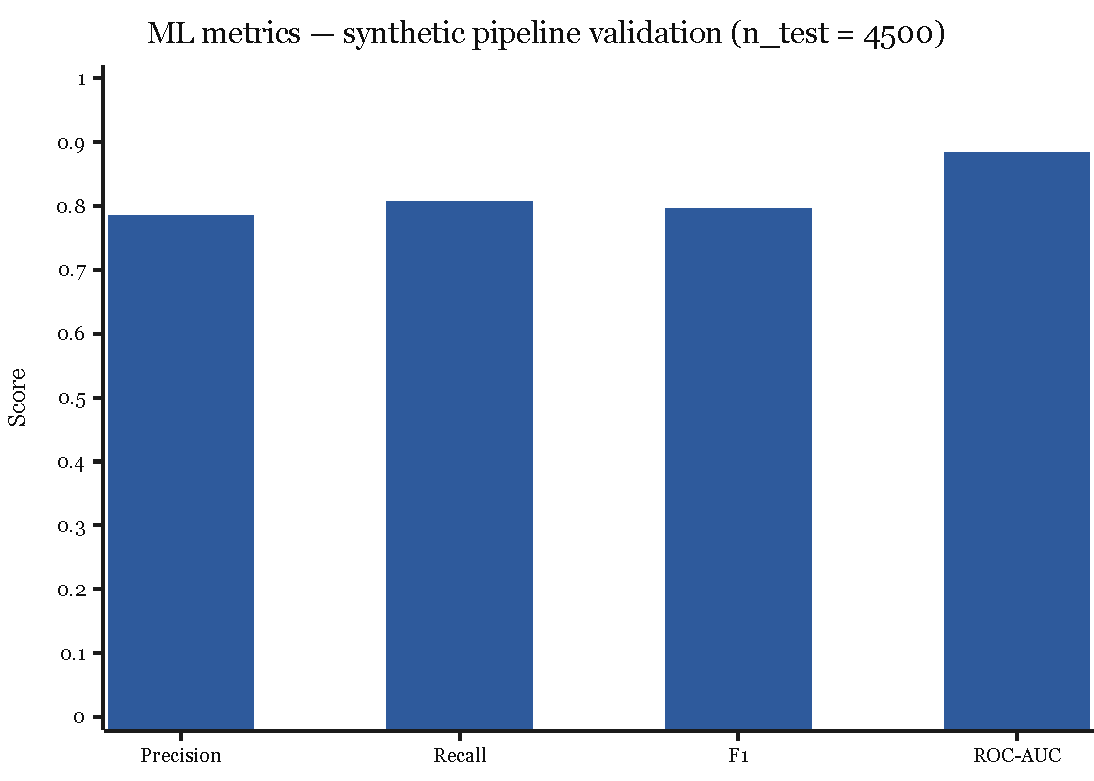
\includegraphics[width=0.50\textwidth,keepaspectratio]{fig-ml-metrics-bars.pdf}
\caption{Off-chain risk model metrics on BCCC-DeFiFraudTrans-2025 (wallet-grouped split).}
\label{fig:ml}
\end{figure}

%----------------------------------------------------------------------
\section{Architecture and Governance}
\label{sec:arch}
% 30 points --- the heaviest section, includes checklist
%----------------------------------------------------------------------

\subsection{Technical architecture and platform choice}

CWB is a four-layer DApp (Figure~\ref{fig:layers}).

\begin{enumerate}
  \item \textbf{Presentation ---} React, TypeScript, WalletConnect / RainbowKit. Retail, approver, reserve, group-lending, and compliance views. Every value-moving action ends in a wallet signature.
  \item \textbf{Application ---} Express.js REST (RBAC, JWT), FastAPI ML (\texttt{/score} $\le$50~ms target), MCP tool server, blockchain event listener.
  \item \textbf{Persistence ---} PostgreSQL projections, append-only audit tables with row-level security, Redis sessions. Not authoritative for balances.
  \item \textbf{On-chain ---} Solidity~0.8.20. Core: World / National / Local Bank contracts, loan controller, savings vault, group pool, interbank pool, upward deposit facility, insurance fund. Specified next: syndicated and tranched pools, treasury swap, liquidation engine.
\end{enumerate}

\begin{figure}[H]
\centering
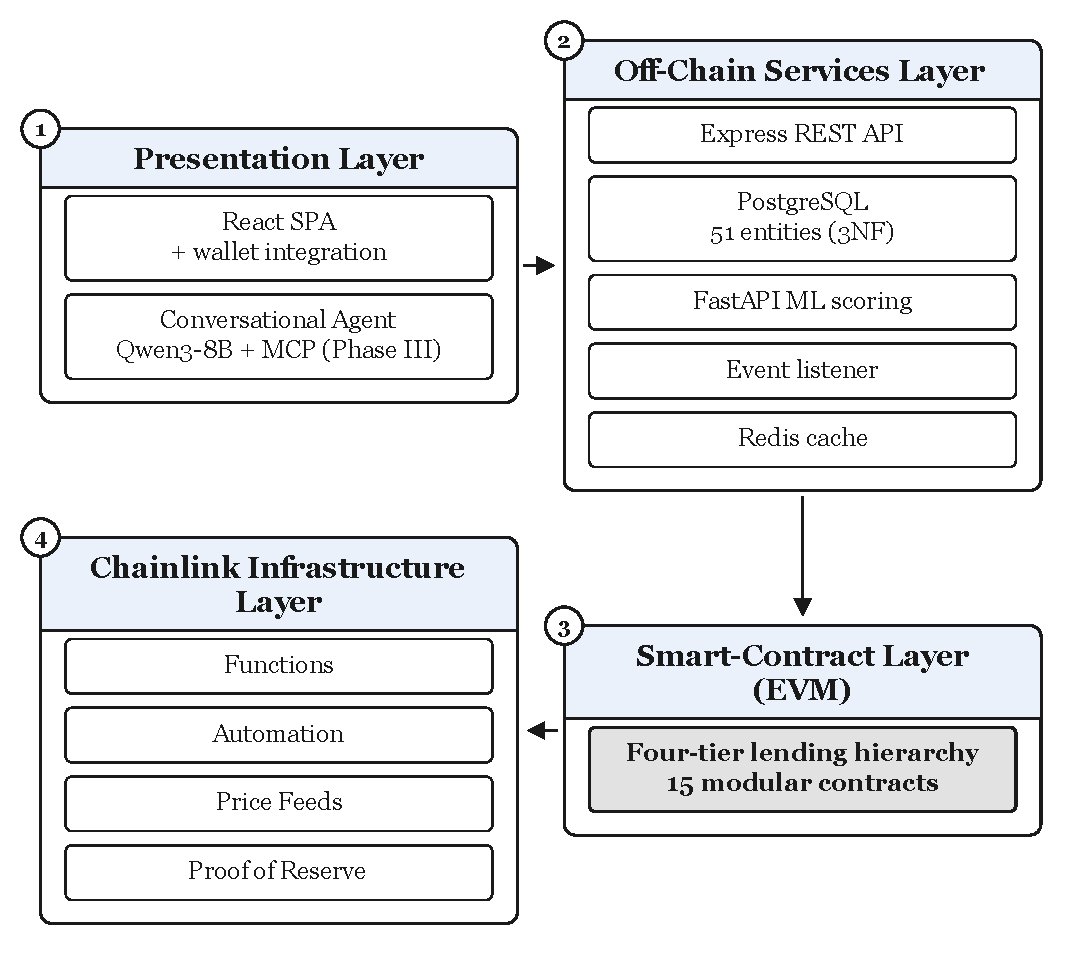
\includegraphics[width=0.55\textwidth,keepaspectratio]{fig-three-layer-arch.pdf}
\caption{Four-layer architecture: UI, services, off-chain data, EVM contracts.}
\label{fig:layers}
\end{figure}

The stack follows an MVC split at repository root: \textbf{Model} is the Solidity state machines plus PostgreSQL projections; \textbf{View} is the React/TypeScript wallet UI; \textbf{Controller} is Express.js. Table~\ref{tab:four-layer} is the design specification used for implementation.

\begin{table}[H]
\centering
\footnotesize
\caption{Four-layer architecture specification.}
\label{tab:four-layer}
\begin{tabular}{@{}>{\raggedright\arraybackslash}p{2.3cm}>{\raggedright\arraybackslash}p{3.4cm}>{\raggedright\arraybackslash}p{3.8cm}>{\raggedright\arraybackslash}p{4.3cm}@{}}
\toprule
\tablehead Layer & Technology & Key components & Responsibility \\
\midrule
Presentation & React, TypeScript, WalletConnect / RainbowKit & Retail, approver, reserve, group, compliance views & User interaction; every value move ends in a wallet signature \\
\rowcolor{RowShade}
Application & Express.js, FastAPI & REST API, ML \texttt{/score}, MCP agent, event listener & Business logic, inference, tool calls, orchestration \\
Persistence & PostgreSQL, Redis & Lending projections, append-only audit, sessions & Off-chain read models synced from chain events; never authoritative for balances \\
\rowcolor{RowShade}
On-chain & Solidity 0.8.20 (EVM) & Tier contracts, \texttt{LoanController}, vaults and pools & Authoritative banking state, RBAC, reserve rules, loan lifecycle \\
\bottomrule
\end{tabular}
\end{table}

\begin{table}[H]
\centering
\footnotesize
\caption{Smart-contract inventory (authoritative on-chain design).}
\label{tab:contracts}
\begin{tabular}{@{}>{\raggedright\arraybackslash}p{3.15cm}>{\raggedright\arraybackslash}p{2.35cm}>{\raggedright\arraybackslash}p{1.55cm}>{\raggedright\arraybackslash}p{6.7cm}@{}}
\toprule
\tablehead Contract & Module & Status & Primary responsibility \\
\midrule
\texttt{WorldBankReserve} & Tier~1 core & Phase~I & Global reserve custody; National Bank registration; downward \texttt{allocateCapital} \\
\rowcolor{RowShade}
\texttt{NationalBank} & Tier~2 core & Phase~I & Local Bank registration; upward borrow; downward allocation \\
\texttt{LocalBank} & Tier~3 core & Phase~I & Client onboarding; approvers; owns \texttt{LoanController}; \texttt{freezeAccount} \\
\rowcolor{RowShade}
\texttt{LoanController} & Lending SM & Phase~II & Request $\to$ score gate $\to$ approve $\to$ disburse $\to$ installment $\to$ repay \\
\texttt{SavingsVault} & Deposits & Phase~II & ERC-4626 variable yield; reserve-gated withdrawals \\
\rowcolor{RowShade}
\texttt{GroupLendingPool} & Group credit & Phase~II & 3--20 members; multi-sig consent; mutual liability; per-member share \\
\texttt{InterBankLendingPool} & Multi-entity & Phase~II & Same-tier 1/7/30-day peer liquidity \\
\rowcolor{RowShade}
\texttt{UpwardDepositFacility} & Multi-entity & Phase~II & Surplus repatriation to parent with $r_{\mathrm{up}}<r_{\mathrm{down}}-\delta$ \\
\texttt{InsuranceFund} & Risk buffer & Phase~I/II & 5\% interest capture; default cover; PoR upgrade path \\
\rowcolor{RowShade}
\texttt{SyndicatedLoan} / \texttt{TranchedPool} & Multi-entity & Phase~III & Multi-bank co-funding; senior/junior waterfall \\
\texttt{TreasurySwap} / \texttt{FXModule} & Treasury & Phase~III & Oracle-priced institutional and retail FX \\
\rowcolor{RowShade}
\texttt{LiquidationEngine} & Risk & Phase~III & Health factor; 5--8\% liquidator bonus when $HF<1$ \\
\texttt{MockUSDC} & Settlement asset & Phase~I & Mintable ERC-20 unit of account on testnet \\
\bottomrule
\end{tabular}
\end{table}

\textbf{Loan state machine.} \texttt{LoanController} is deployed by each Local Bank. A request enters \texttt{PENDING\_SCORE}; the oracle commit--reveal must succeed before the approver key can move it to approved or rejected; disbursement writes \texttt{ACTIVE} and materialises the installment schedule; repayment, overdue checks, or $HF<1$ liquidation are subsequent transitions. Rolling six-month and one-year borrowing caps are computed off-chain and enforced on-chain via \texttt{LocalBank.updateBorrowingLimit}. Reserve-ratio checks revert \texttt{allocateCapital} and vault withdrawals at every tier before funds move.

\subsubsection{Transaction lifecycle (frontend to confirmed state)}

A client action is not an API side-effect. Path:

\begin{enumerate}
  \item \textbf{UI $\to$ gateway.} React (Wagmi/RainbowKit/Viem) validates the form, attaches the connected address, and calls Express. Middleware order: JWT / wallet auth, schema validation, rate limit. Read-only calls stop here.
  \item \textbf{Calldata and signing.} The gateway or the browser encodes the function selector and arguments. EIP-712 typed data is used for login; value-moving calls are signed by the client wallet (or, later, an EIP-7702 session key with on-chain scope). The ML path additionally commits $h=\mathrm{keccak256}(s\|\mathrm{nonce})$ before reveal.
  \item \textbf{Mempool to block.} The signed transaction is submitted to Sepolia or Amoy. Public PoS validators propose and attest; CWB runs no private notary, orderer, or Fabric peer set. Contract storage updates (reserves, loan enum, roles) and events (\texttt{LoanRequested}, \texttt{Disbursed}, \texttt{Repaid}, \texttt{CapitalAllocated}) are the source of truth. Frontend waits for configured confirmation depth.
  \item \textbf{Projection.} The event listener is the only writer of lending projection tables. It upserts \texttt{BLOCKCHAIN\_EVENT\_LOG} by \texttt{tx\_hash} and fans out to \texttt{LOAN}, \texttt{INSTALLMENT}, \texttt{CREDIT\_PASSPORT}. If cache and chain disagree, chain wins.
\end{enumerate}

Gas on the L2/testnet design path is \$0.001--\$0.01 per step and $\approx$\$0.011 for a 27--32-step retail lifecycle---below 0.01\% of interest on the \$25{,}000 planning ticket---which is why EVM L2 is preferred over L1 retail and over a permissioned Fabric channel that would hide the reserve from the public.

\subsubsection{Why a public EVM (and not Fabric, Corda, or a private chain)}

\begin{table}[H]
\centering
\small
\caption{Platform decision (technology assessment and adoption).}
\label{tab:platform}
\begin{tabular}{@{}>{\raggedright\arraybackslash}p{3.1cm}>{\raggedright\arraybackslash}p{4.4cm}>{\raggedright\arraybackslash}p{6.3cm}@{}}
\toprule
\tablehead Option & Verdict & Reason \\
\midrule
Hyperledger Fabric (orderers, peers, channels) & Rejected as primary & Club trust; parent can still be the consortium operator; weaker public audit for development funds \\
\rowcolor{RowShade}
Corda (notary network) & Rejected as primary & Excellent for bilateral trade privacy; poor fit for \textit{public} reserve transparency the lower tier must verify \\
Permissioned Ethereum / Quorum & Fallback & If a sandbox demands validator allow-lists; same Solidity, weaker public verifiability \\
\rowcolor{RowShade}
Solana / non-EVM & Rejected & Weaker OpenZeppelin-class contract security corpus for this team and timeline \\
\textbf{Public EVM PoS} (Sepolia now; Amoy secondary; zkEVM design target) & \textbf{Selected} & Independent verification; mature RBAC libraries; free testnets; L2 gas compatible with MSME tickets; PoS $\approx$99.9\% less energy than PoW \\
\bottomrule
\end{tabular}
\end{table}

\textbf{Consensus and transaction verification.} Prototype networks are Ethereum Sepolia (PoS testnet) and Polygon Amoy. Blocks are proposed and attested by the public validator set of that network; CWB does not run a private notary. Finality on the L2 design path is on the order of two seconds, which is acceptable for branch UX. Production intent is a zkEVM so validity proofs inherit L1 security without putting retail gas on L1. \textbf{Multi-chain bridges are out of scope} after explicit rejection of bridge-attack surface.

\begin{table}[H]
\centering
\footnotesize
\caption{Selected platform parameters (technology assessment).}
\label{tab:platparams}
\begin{tabular}{@{}>{\raggedright\arraybackslash}p{3.2cm}>{\raggedright\arraybackslash}p{4.2cm}>{\raggedright\arraybackslash}p{6.4cm}@{}}
\toprule
\tablehead Criterion & Selection & Justification \\
\midrule
Platform / language & EVM, Solidity 0.8.20 & Overflow-safe compiler; OpenZeppelin RBAC, CEI, pause; portable across EVM chains \\
\rowcolor{RowShade}
Networks & Sepolia primary; Amoy secondary & Free public testnets; zkEVM Cardona is the design target, not the day-one demo chain \\
Consensus & Public PoS (testnet validators) & Independently verifiable; no CWB-operated orderer/notary \\
\rowcolor{RowShade}
Finality / gas & $\approx$2~s L2; \$0.001--\$0.01 / tx & Retail UX; micro-loan viable; L1 same lifecycle costs \$2.40--\$4.80 \\
Tooling & Hardhat + Foundry + OpenZeppelin & 42 Hardhat cases now; Foundry invariants (solvency, role segregation, capital-flow direction) in verification \\
\rowcolor{RowShade}
Oracle (MVT) & Commit--reveal relay & Always available; Chainlink Functions DON is the production upgrade \\
\bottomrule
\end{tabular}
\end{table}

\subsubsection{On-chain vs.\ off-chain data}

\begin{figure}[H]
\centering
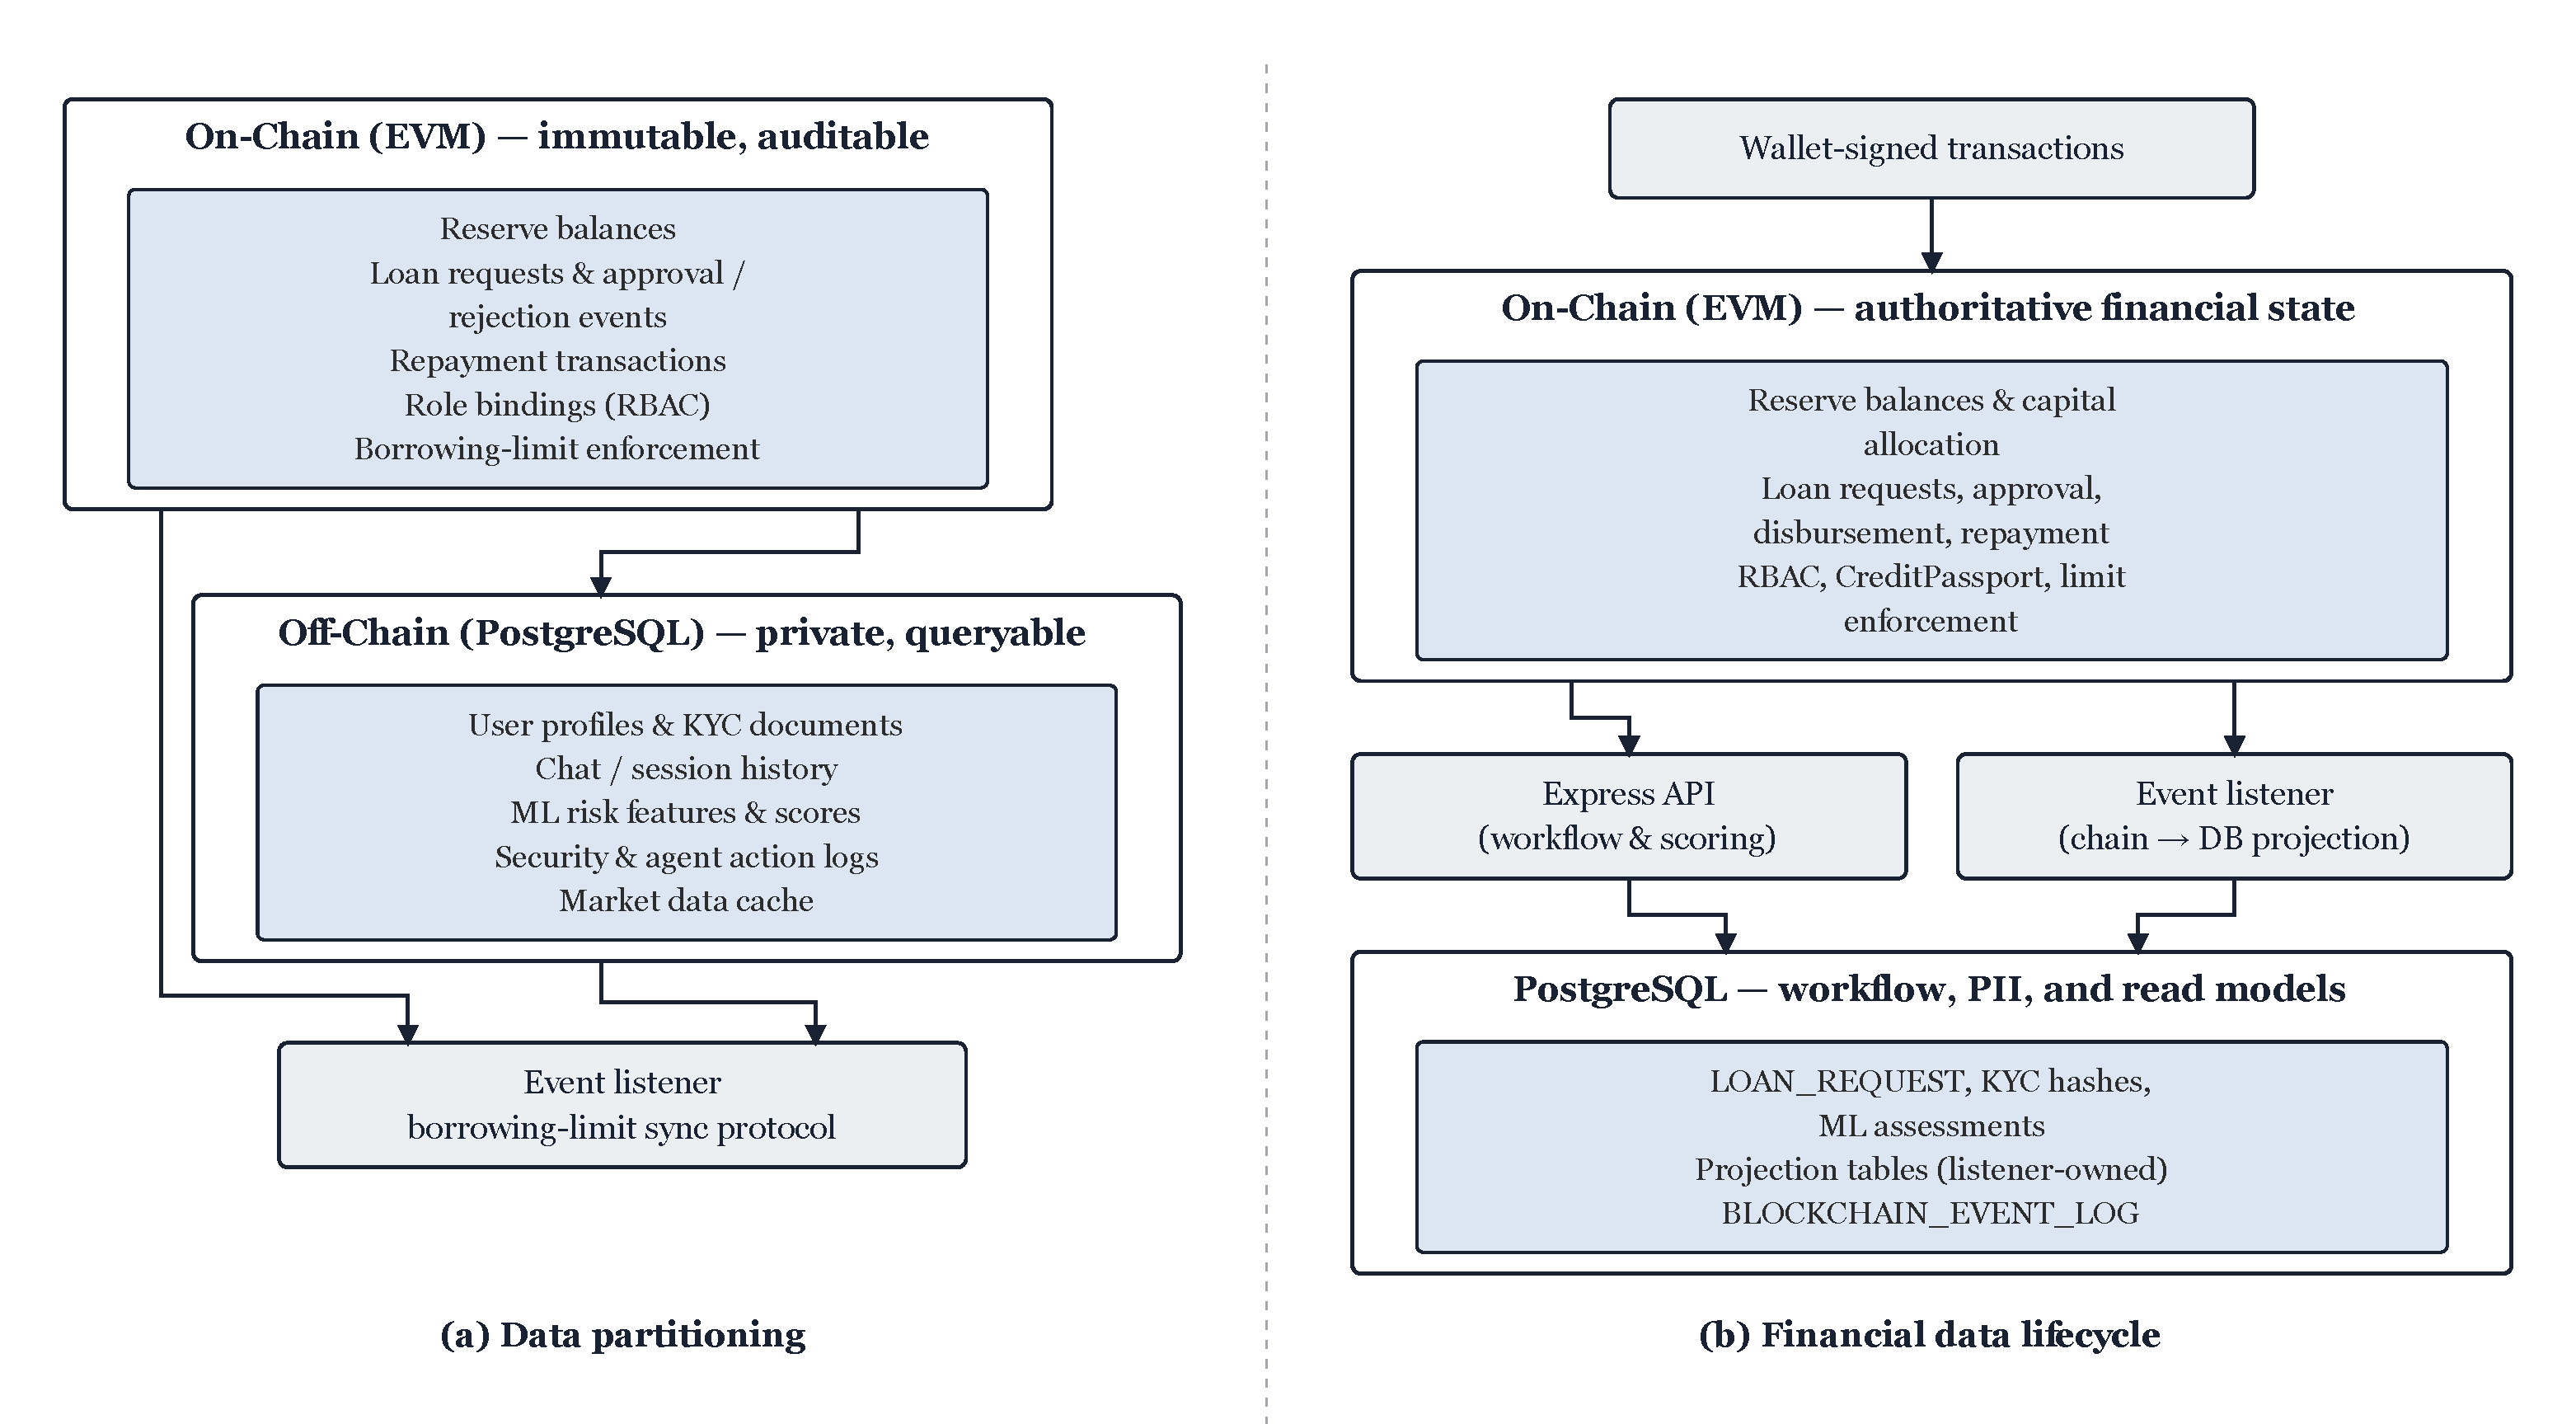
\includegraphics[width=0.90\textwidth,keepaspectratio]{fig-data-partitioning-and-lifecycle.pdf}
\caption{Authoritative balances and roles on-chain; PII, documents, and ML features off-chain.}
\label{fig:partition}
\end{figure}

\textbf{On-chain:} reserve balances, role grants, loan state machine, disbursement and repayment events, group membership and consent, SBT score/tier, pause flags, committed ML score hashes, insurance fund balance. \textbf{Off-chain:} KYC images, income PDFs, chat, SHAP payloads, full ML feature vectors, session keys, agent transcripts. Borrowing-limit \textit{computation} is off-chain (window queries); the resulting cap is written on-chain and enforced there. Chainlink rounds, when enabled, are authoritative on-chain with an off-chain cache for staleness checks.

This split is how a regulated credit product avoids leaking identity while still proving that money moved under published rules.

\begin{table}[H]
\centering
\footnotesize
\caption{On-chain / off-chain partition (data services).}
\label{tab:partition}
\begin{tabular}{@{}>{\raggedright\arraybackslash}p{4.6cm}p{2.2cm}>{\raggedright\arraybackslash}p{6.9cm}@{}}
\toprule
\tablehead Data & Storage & Rationale \\
\midrule
Reserves, loan events, repayments, RBAC, SBT score/tier & On-chain & Immutability; any party can verify without asking the operator \\
\rowcolor{RowShade}
Profiles, KYC images, chat, SHAP vectors, agent transcripts & Off-chain DB & Privacy, query cost; only hashes and role flags hit calldata \\
Borrowing-limit windows & Off-chain compute, on-chain cap & Temporal aggregation is expensive on-chain; \texttt{updateBorrowingLimit} is authoritative \\
\rowcolor{RowShade}
Price / PoR rounds & On-chain feed + cache & \texttt{AggregatorV3Interface} authoritative; cache detects staleness \\
\texttt{AGENT\_ACTION\_LOG} & Off-chain append-only & Linked to \texttt{tx\_hash}; RLS forbids UPDATE/DELETE \\
\bottomrule
\end{tabular}
\end{table}

\paragraph{Data model.}
The off-chain schema is specified in 3NF with 51 entities; the prototype ships 16 Must (M1) tables. Hierarchy uses table-per-type specialisation: \texttt{INSTITUTION} is the shared identity; \texttt{WORLD\_BANK} (singleton \texttt{institution\_id}=1), \texttt{NATIONAL\_BANK} (unique \texttt{country\_code}), and \texttt{LOCAL\_BANK} are subtypes. Actors: \texttt{BANK\_USER} (exactly one parent institution by CHECK) and \texttt{BORROWER} (unique \texttt{wallet\_address}, mandatory home Local Bank, hash-only KYC). Lending: \texttt{LOAN\_REQUEST} $\to$ \texttt{LOAN} $\to$ weak entity \texttt{INSTALLMENT}. Sync: \texttt{BLOCKCHAIN\_EVENT\_LOG} is the canonical event cache and FK target for disbursement linkage. Integrity: UNIQUE on contract addresses and tx hashes; append-only RLS on \texttt{AUDIT\_LOGS}, \texttt{SECURITY\_EVENT\_LOG}, \texttt{AGENT\_ACTION\_LOG}; event-listener-only write on \texttt{CREDIT\_PASSPORT} and \texttt{BORROWING\_LIMIT} projections. Phase~II+ adds group, interbank, savings, model registry, and session lineage tables without moving PII on-chain.

Digital identity is therefore three-layer: wallet authentication (MetaMask / WalletConnect + EIP-712 login), off-chain Level~1/2 KYC store, and a soulbound Credit Passport. A regulator receives a read-only event package; they do not receive the KYC image store unless a lawful process demands it off-chain.

\subsubsection{Tokenisation model}

\begin{itemize}
  \item \textbf{Settlement asset ---} ERC-20 stablecoin (testnet \texttt{MockUSDC}). Tokenises the unit of account, not land or invoices, in the MVT.
  \item \textbf{Savings shares ---} ERC-4626 vault tokens. Depositors hold a claim on the pool; withdrawals revert if they would breach the tier reserve ratio.
  \item \textbf{Identity / reputation ---} Credit Passport as a soulbound (non-transferable) token. Score 0--1000 maps to Bronze through Diamond. Bronze max loan 50~USDC; Diamond 25{,}000~USDC with rate discounts up to 2\%. It cannot be sold, so mule markets cannot buy a Diamond identity.
  \item \textbf{Group credit ---} membership and mutual liability inside \texttt{GroupLendingPool}; default hits shared collateral then SBT downgrade, not a secret office spreadsheet.
  \item \textbf{Future ---} Groth16 zkKYC (possession of a credential without PII on-chain) is specified, not claimed as shipped.
\end{itemize}

\begin{figure}[H]
\centering
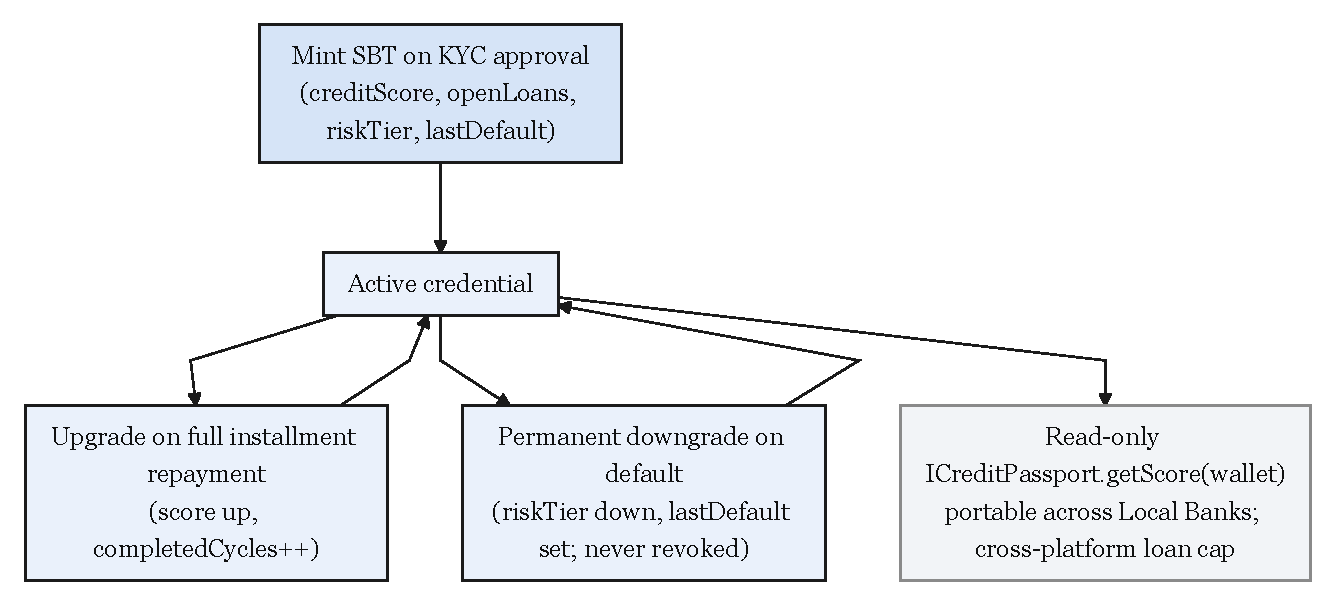
\includegraphics[width=0.58\textwidth,keepaspectratio]{fig-credit-passport.pdf}
\caption{Credit Passport lifecycle: soulbound reputation without on-chain PII.}
\label{fig:sbt}
\end{figure}

\subsubsection{Programmable banking modules}

Retail interest follows a kinked utilisation curve (Figure~\ref{fig:kink}): below $U^*=80\%$ credit is cheap; above the kink the rate jumps so a pool cannot be emptied at the overnight price. Same-tier banks that are long cash lend to peers through \texttt{InterBankLendingPool} (Figure~\ref{fig:ib}) at $r_{\mathrm{IB}}(U)\le r_{\mathrm{down}}(U)-\delta$ instead of parking idle correspondent balances. Surplus at a child bank can be repatriated through \texttt{UpwardDepositFacility} at a strictly lower rate than downward credit, which is the on-chain analogue of a development-bank deposit facility. \texttt{SavingsVault} (ERC-4626) splits collected interest among depositor yield, a 5\% \texttt{InsuranceFund} slice, and protocol revenue; withdrawals revert if they would breach the reserve ratio (Figure~\ref{fig:vault}). Under-collateralised positions are monitored by \texttt{LiquidationEngine}: when health factor $HF<1$, independent liquidators earn a 5--8\% bonus; group loans first consume shared collateral, then downgrade the SBT rather than silently rolling the loss into a parent.

\begin{figure}[H]
\centering
\begin{minipage}[t]{0.48\textwidth}
\centering
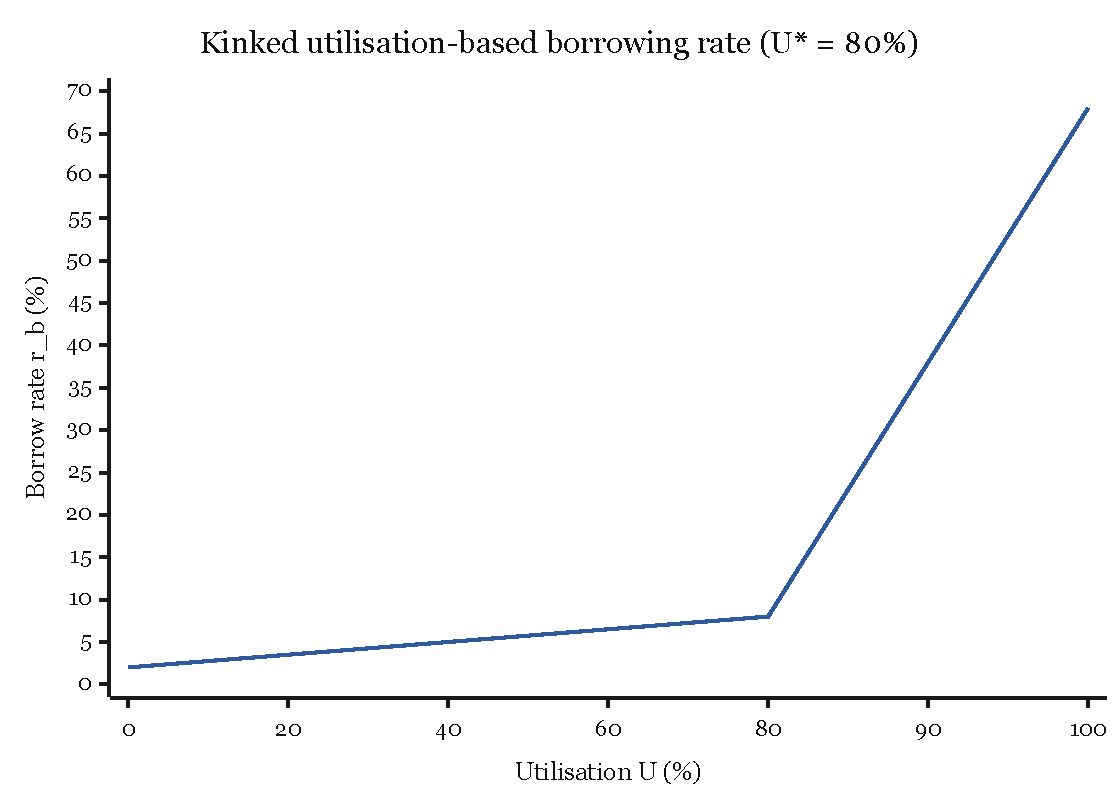
\includegraphics[width=\linewidth,keepaspectratio]{fig-kinked-rate-curve.pdf}
\caption{Kinked borrow rate at $U^*=80\%$.}
\label{fig:kink}
\end{minipage}\hfill
\begin{minipage}[t]{0.48\textwidth}
\centering
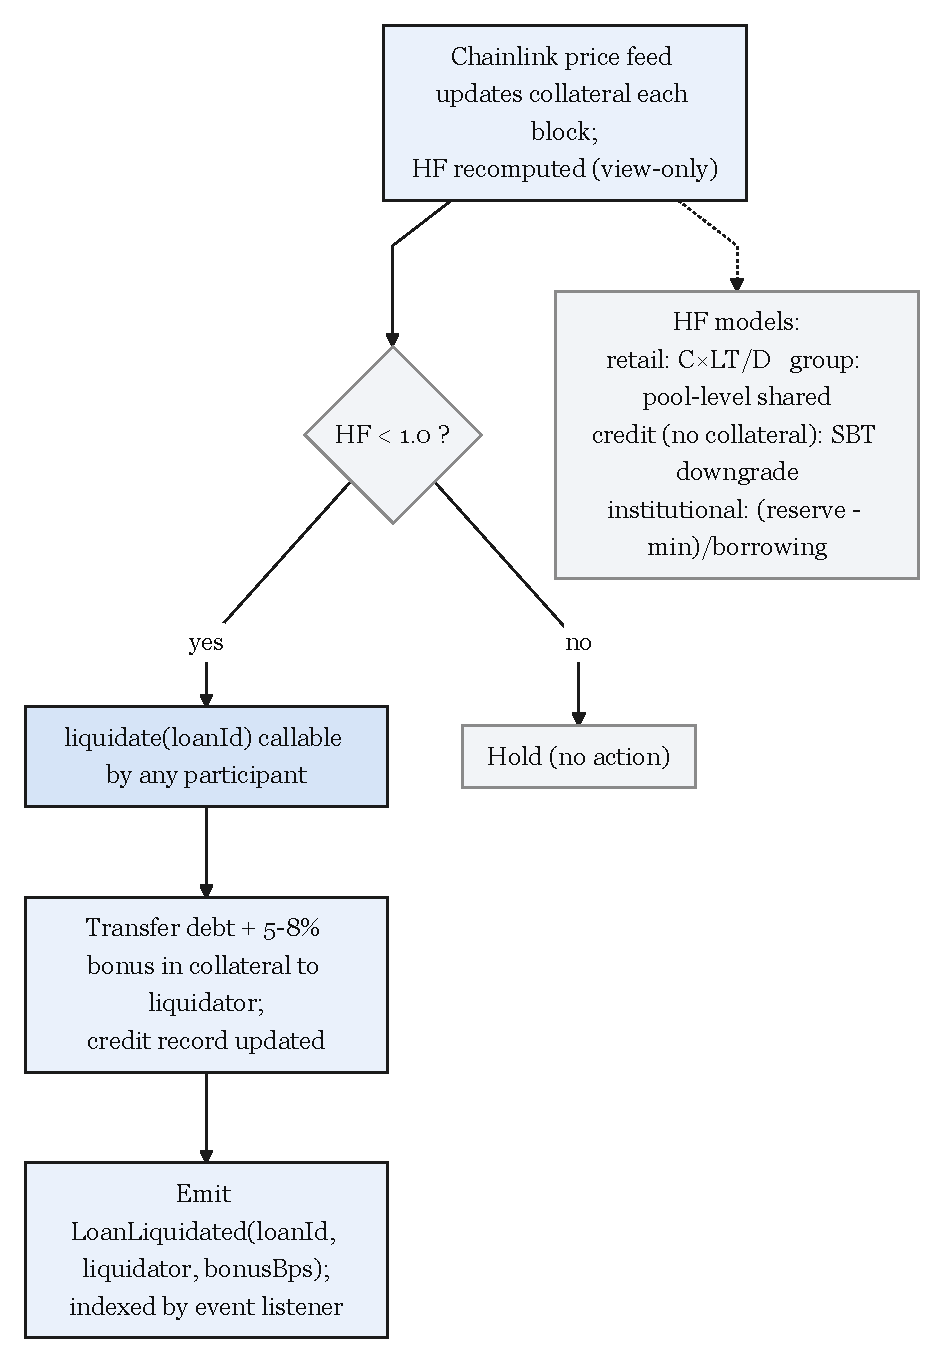
\includegraphics[width=\linewidth,keepaspectratio]{fig-liquidation-engine.pdf}
\caption{Health-factor liquidation with liquidator bonus.}
\label{fig:liq}
\end{minipage}
\end{figure}

\begin{figure}[H]
\centering
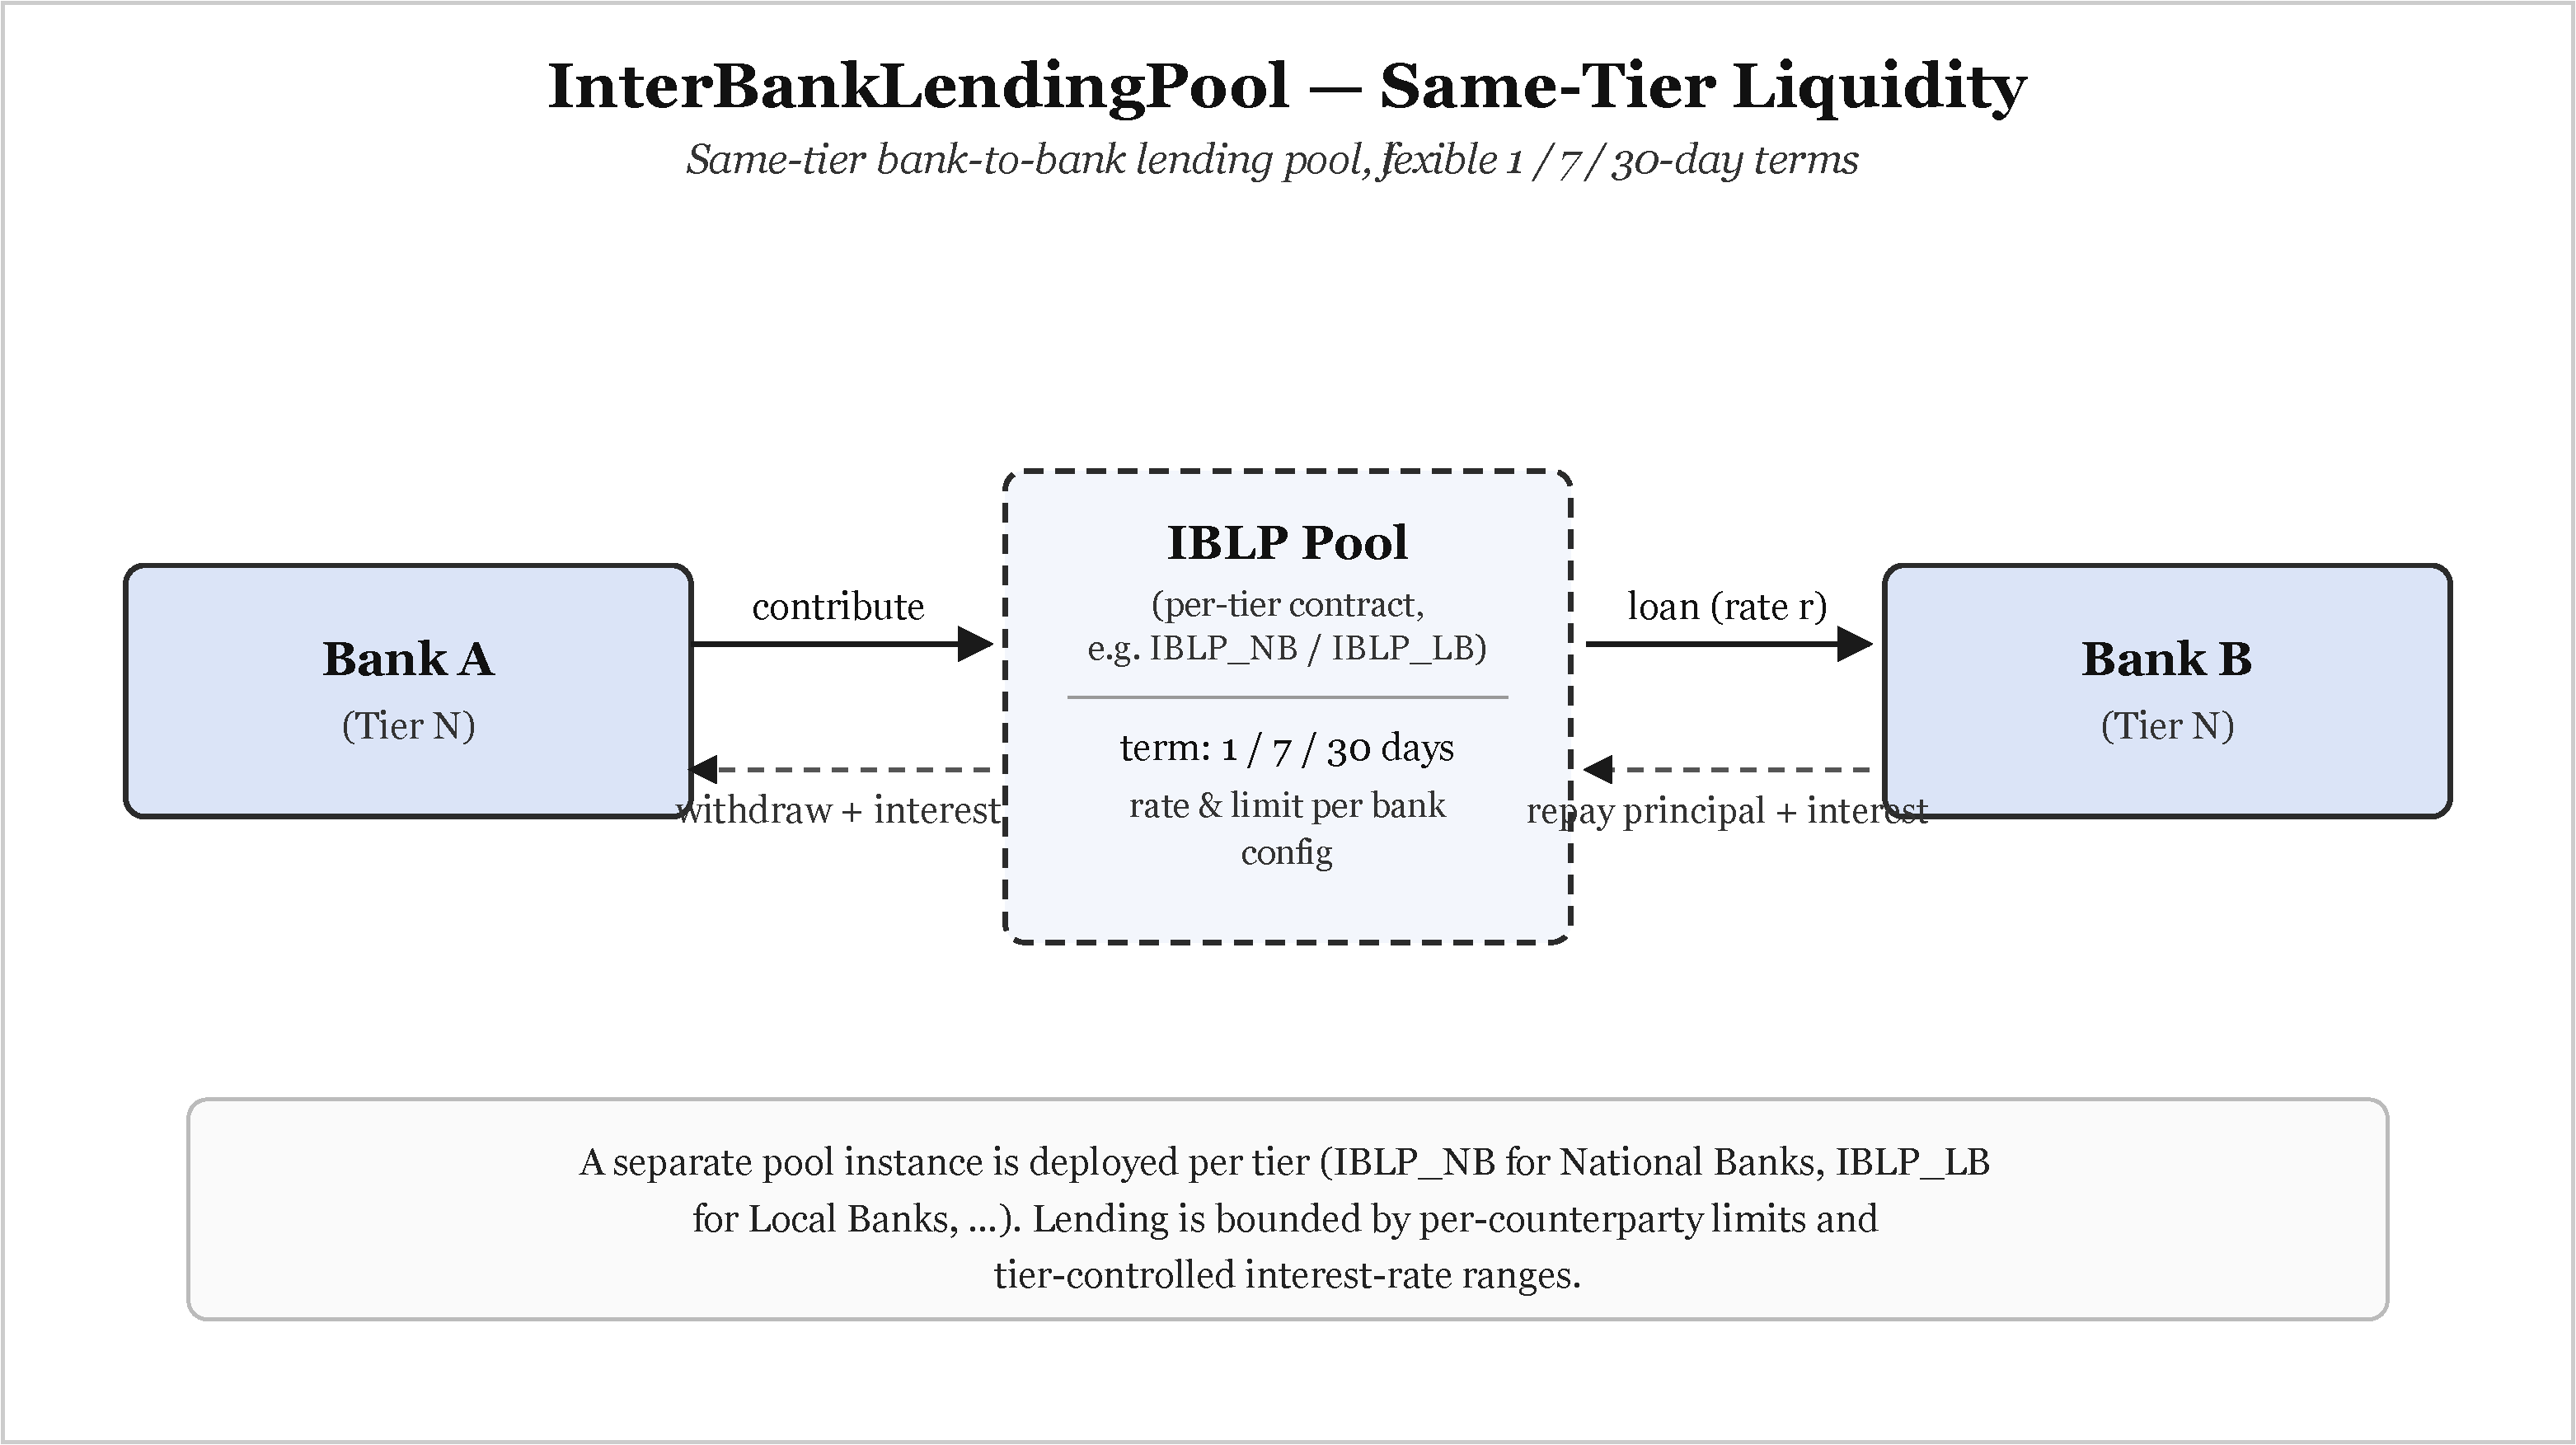
\includegraphics[width=0.82\textwidth,keepaspectratio]{1_InterBankLendingPool_updated.pdf}
\caption{Same-tier \texttt{InterBankLendingPool}: peer liquidity without climbing the parent.}
\label{fig:ib}
\end{figure}

\begin{figure}[H]
\centering
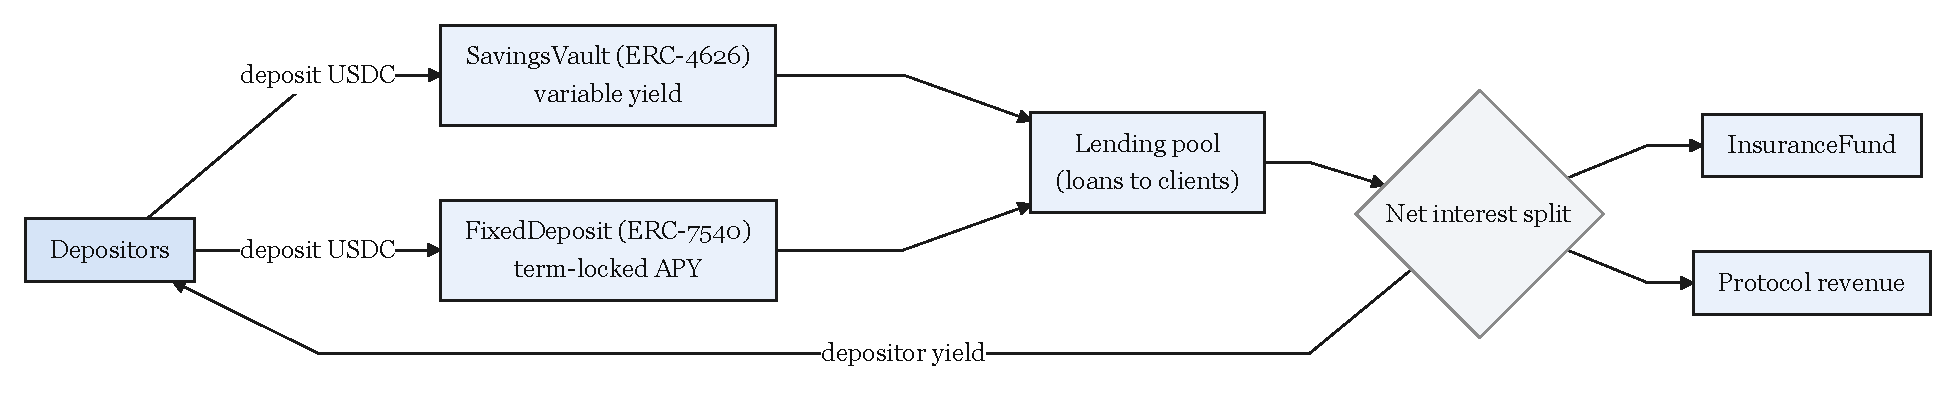
\includegraphics[width=0.82\textwidth,keepaspectratio]{fig-savings-vault.pdf}
\caption{\texttt{SavingsVault}: depositor yield, insurance capture, and reserve-gated exits.}
\label{fig:vault}
\end{figure}

\subsubsection{Oracle, rates, and legacy integration}

Off-chain ML never writes a score in plaintext until reveal (Figure~\ref{fig:oracle}). Table~\ref{tab:chainlink} is the production upgrade map. MVT substitutes keep the same \texttt{LoanController} ABI, so Chainlink can replace the relay without redesigning the loan state machine.

\begin{table}[H]
\centering
\footnotesize
\caption{Oracle and automation: production role versus MVT substitute.}
\label{tab:chainlink}
\begin{tabular}{@{}>{\raggedright\arraybackslash}p{2.8cm}>{\raggedright\arraybackslash}p{5.4cm}>{\raggedright\arraybackslash}p{5.6cm}@{}}
\toprule
\tablehead Service & Production role & MVT / demo substitute \\
\midrule
Chainlink Functions & DON-signed fetch of ML risk score & Commit--reveal relay (authoritative at MVT) \\
\rowcolor{RowShade}
Chainlink Automation & Overdue installments and interest accrual & Node.js cron calling \texttt{checkOverdueLoans()} \\
Price feeds & \texttt{FXModule} / fiat UI via \texttt{AggregatorV3Interface} & \texttt{MockPriceFeed.sol} with fixed testnet answers \\
\rowcolor{RowShade}
Proof of Reserve & External attestation of \texttt{WorldBankReserve} & On-chain \texttt{getReserveSummary()} view \\
\bottomrule
\end{tabular}
\end{table}

Rates and interbank spreads are those of the modules above.

\textbf{Legacy systems.} Core banking does not get replaced. The event listener projects contract events into PostgreSQL so a bank can keep its own MIS, AML vendor, and general ledger. WalletConnect is the customer channel; ISO-style exports are a sandbox integration task, not a new chain. Digital identity is wallet + off-chain KYC hash + SBT---W3C VC/zkKYC later.

\begin{figure}[H]
\centering
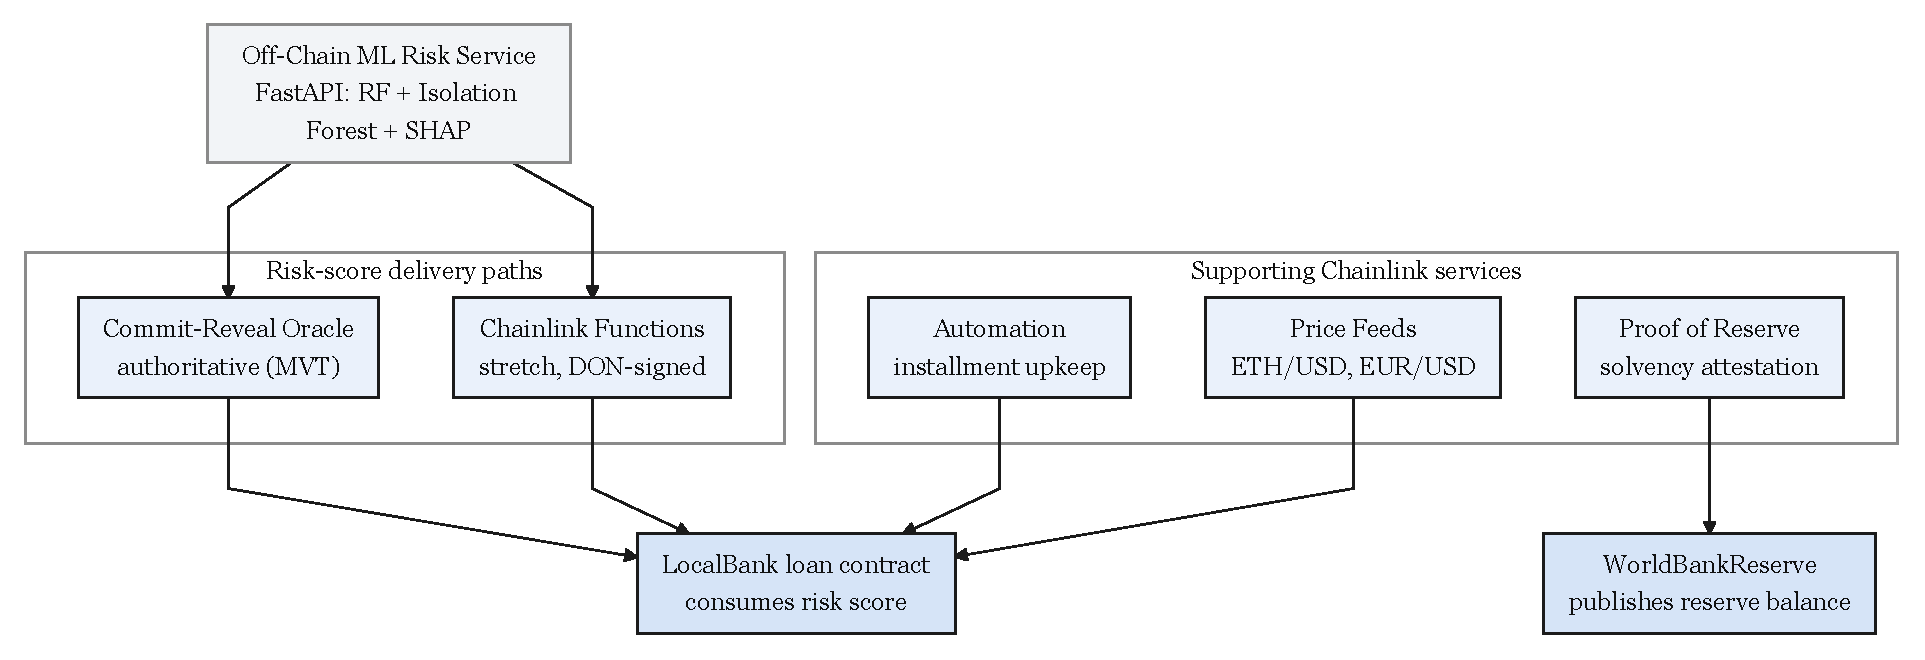
\includegraphics[width=0.82\textwidth,keepaspectratio]{fig-oracle-architecture.pdf}
\caption{Oracle path: off-chain inference, on-chain commit--reveal, human approval.}
\label{fig:oracle}
\end{figure}

\begin{figure}[H]
\centering
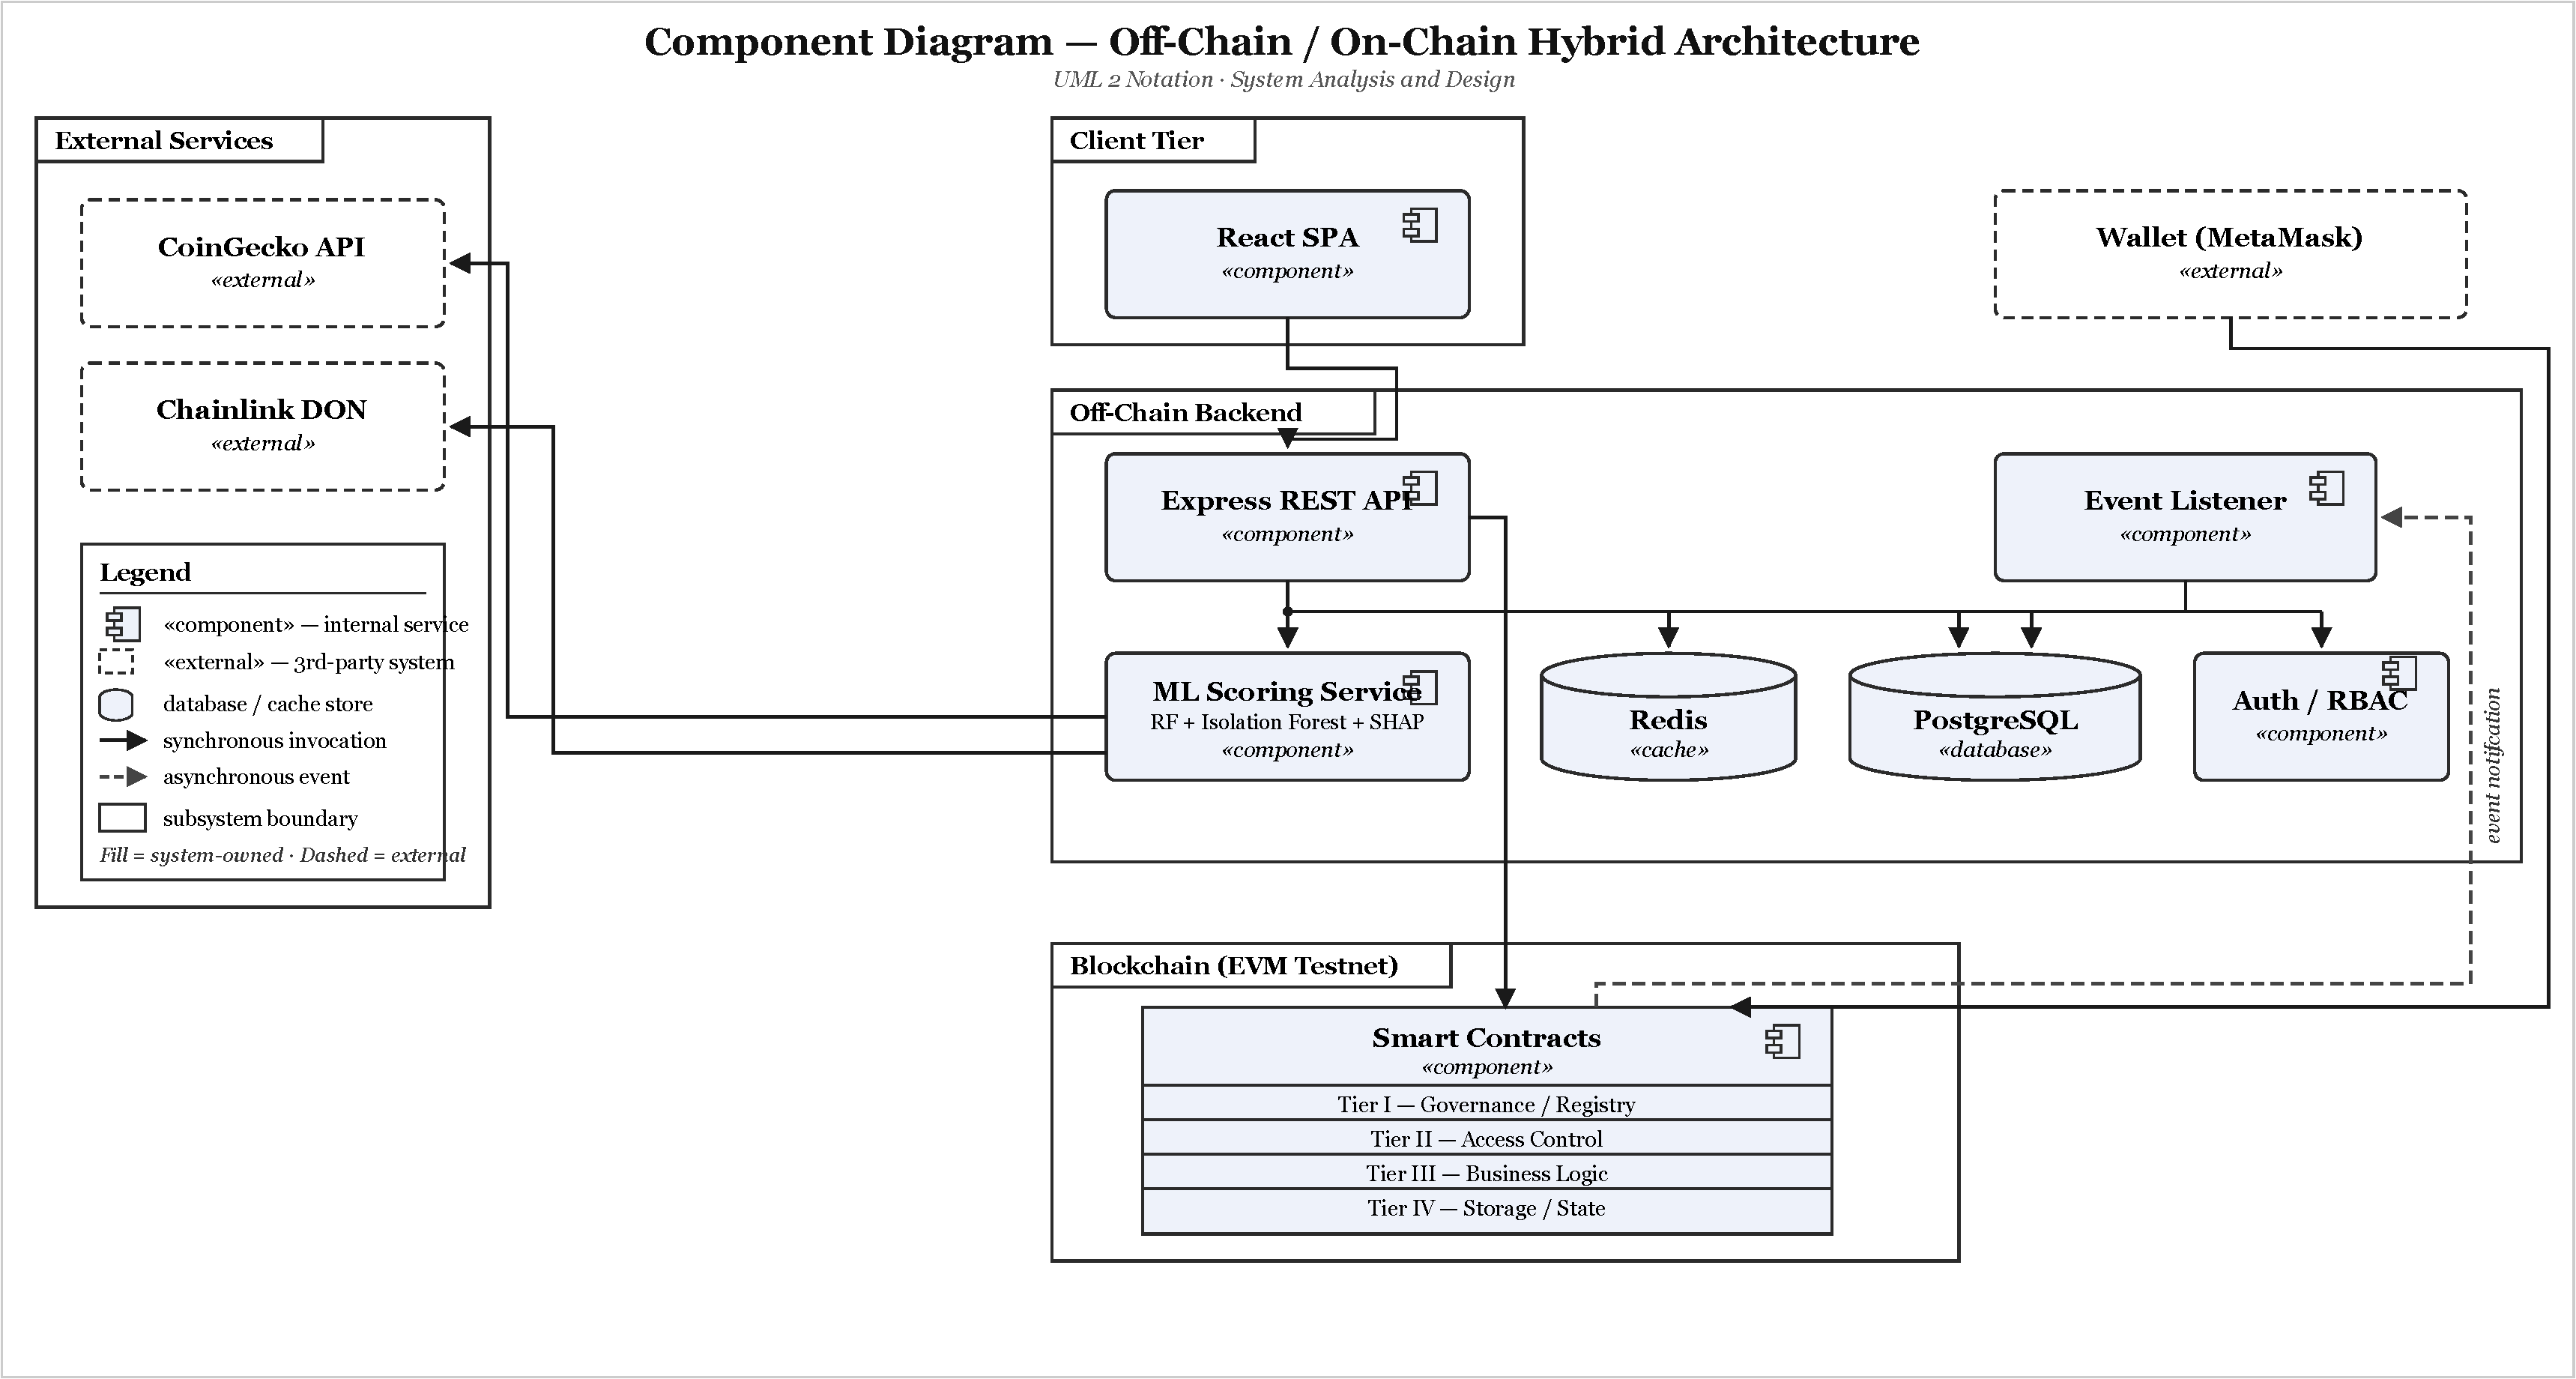
\includegraphics[width=0.80\textwidth,keepaspectratio]{fig-component-architecture_updated.pdf}
\caption{Component interaction among wallets, API, ML, listener, and contracts.}
\label{fig:components}
\end{figure}

\begin{figure}[H]
\centering
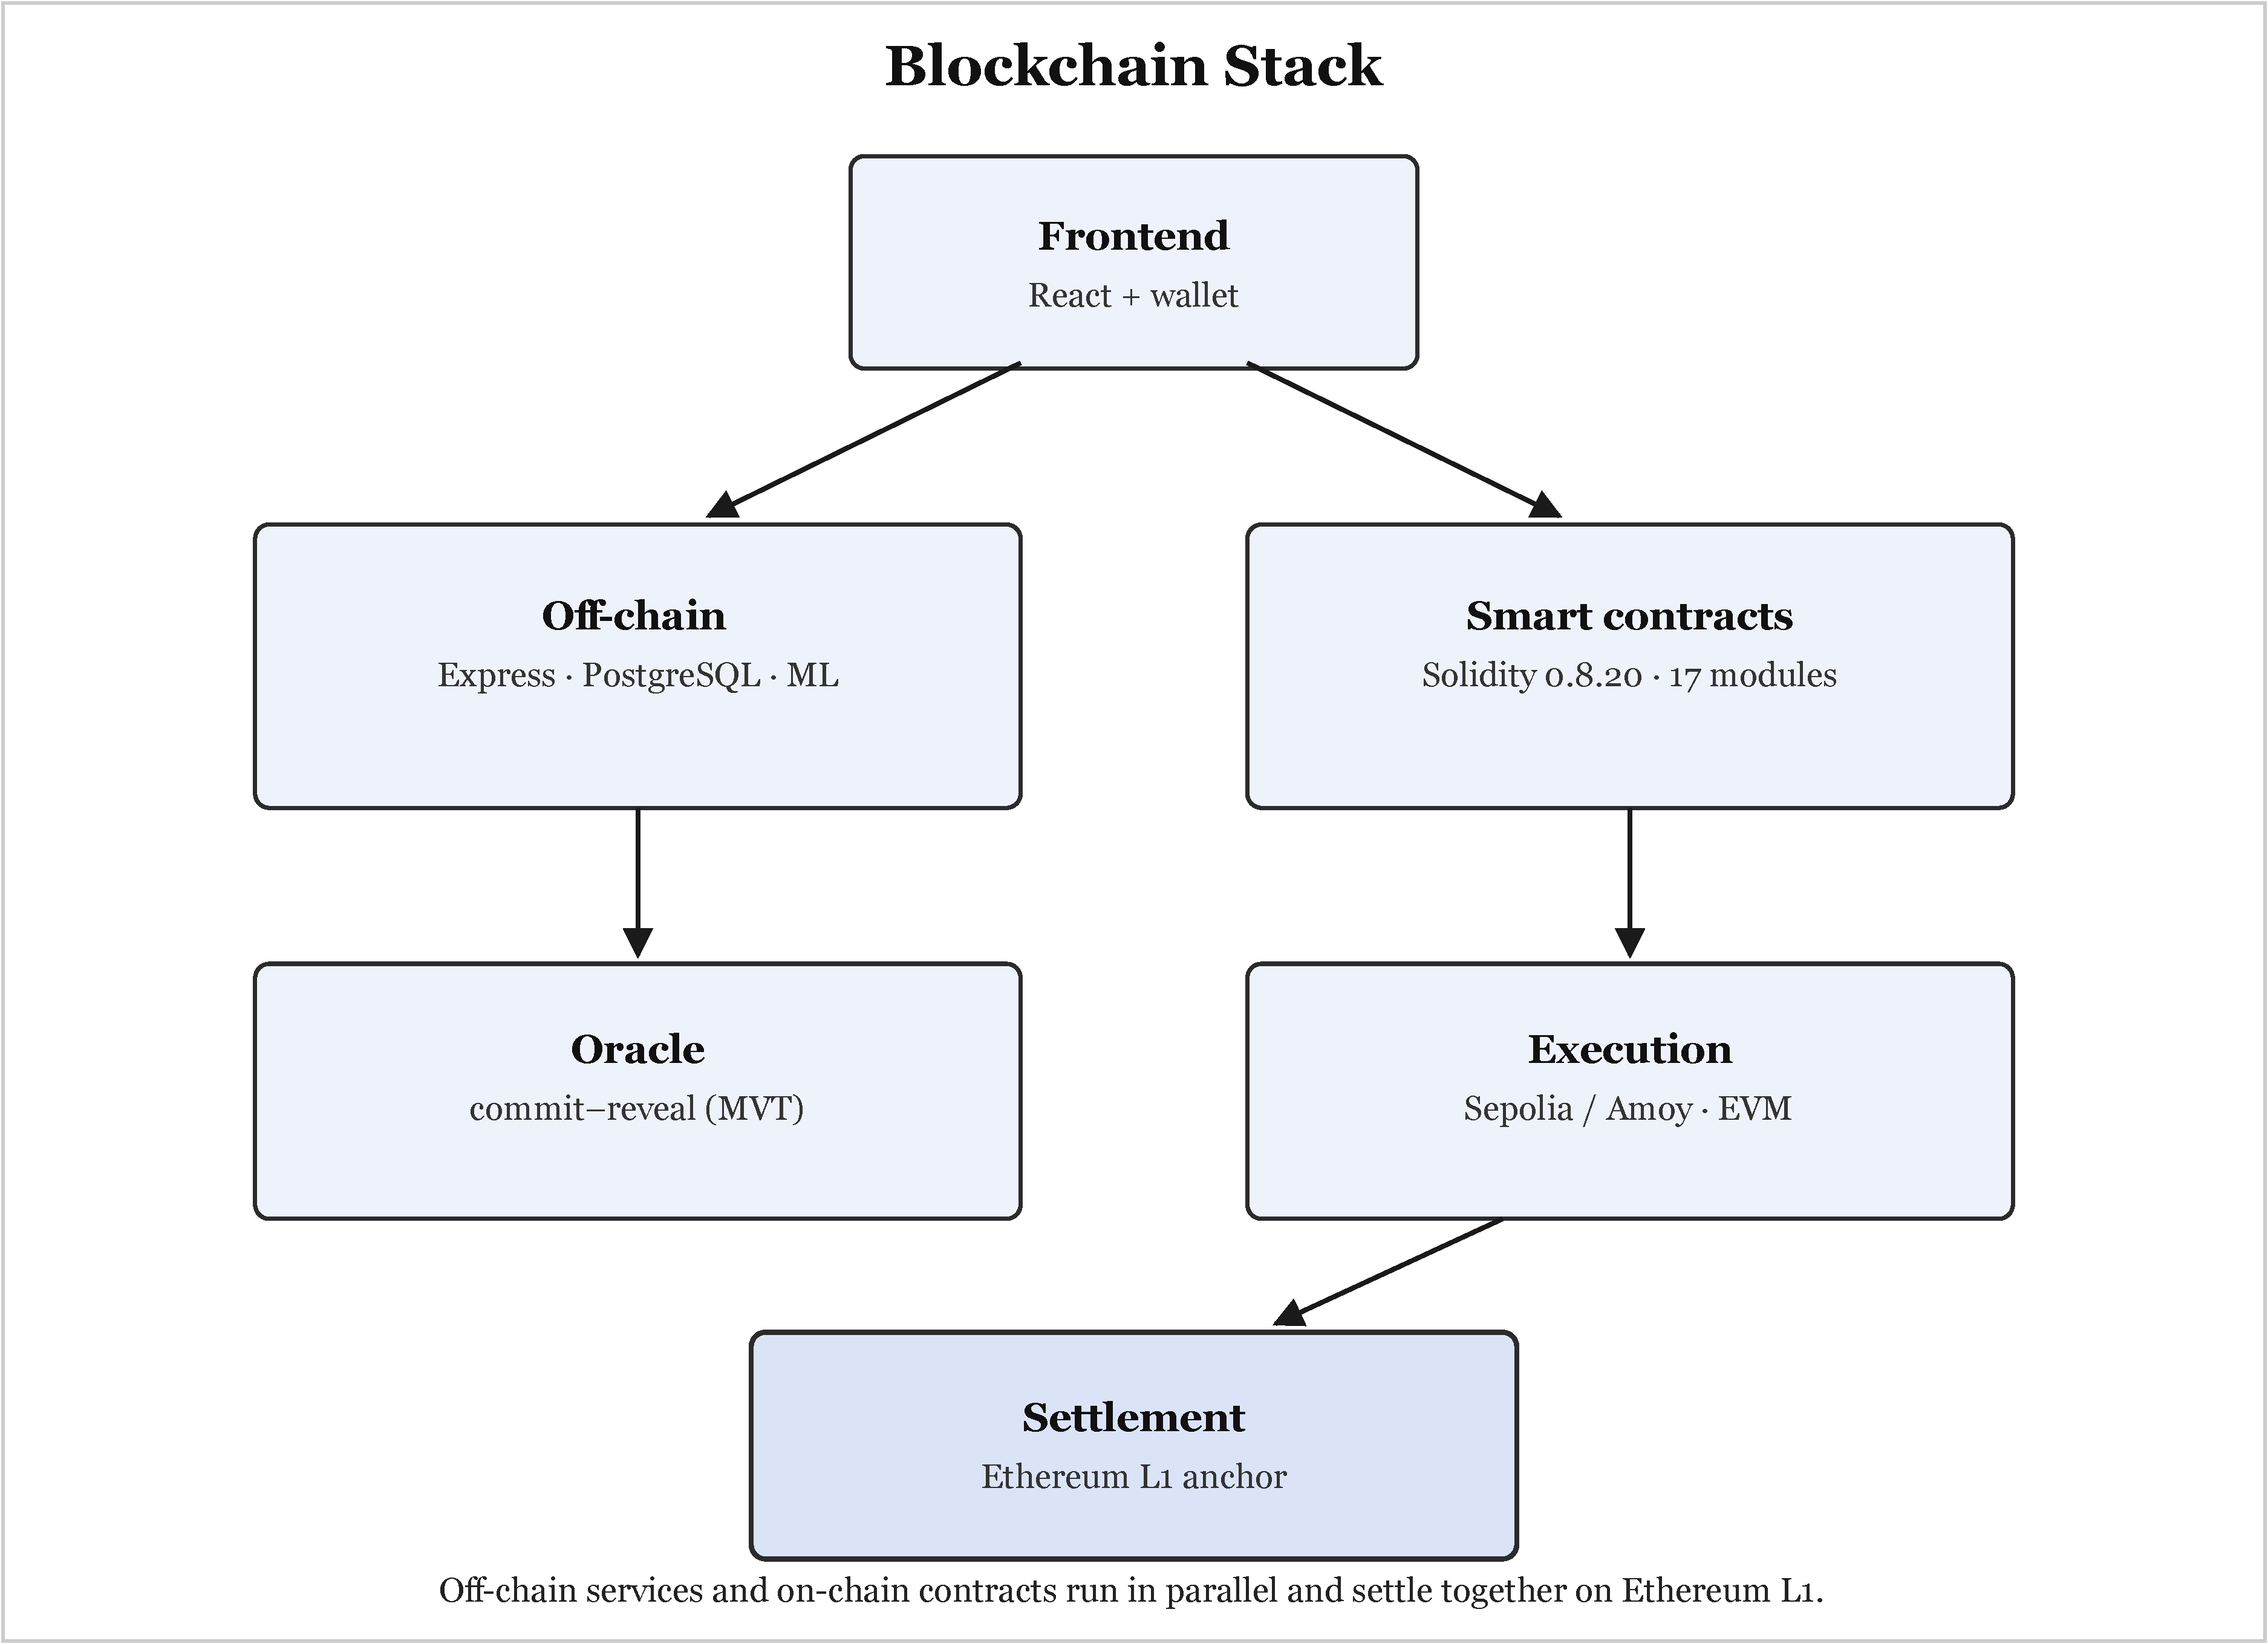
\includegraphics[width=0.78\textwidth,keepaspectratio]{fig-blockchain-stack_updated.pdf}
\caption{Selected blockchain stack: Solidity, OpenZeppelin, Hardhat/Foundry, PoS EVM.}
\label{fig:stack}
\end{figure}

\subsection{Privacy, security, and access control}

Five-layer defense-in-depth (Figure~\ref{fig:defense}):

\begin{itemize}
  \item \textbf{L1 Contracts ---} RBAC, \texttt{ReentrancyGuard}, pause, CEI, UUPS only behind Safe.
  \item \textbf{L2 Application ---} short-TTL JWT, rate limits, prompt-injection scan on agent input.
  \item \textbf{L3 AI/ML ---} RF+IF+SHAP; commit--reveal; never auto-disburse.
  \item \textbf{L4 Monitoring ---} Tenderly-style alerts on large disbursement, low reserve, pause.
  \item \textbf{L5 Operations ---} Safe 2-of-3 for \texttt{WorldBankAdmin}; no lone EOA.
\end{itemize}

\textbf{Data privacy.} PII never enters calldata. Unauthorised parties see public reserve and loan \textit{state}, not income documents. \textbf{Identity privacy.} Wallet addresses are pseudonymous; linkage to a person lives in the bank's KYC store. \textbf{Key management.} Institutions use Safe; retail uses MetaMask/WalletConnect; agent writes require a fresh human signature (EIP-7702 session keys are stretch). \textbf{Access control.} Table~\ref{tab:perms} is enforced in Solidity modifiers \textit{and} API RBAC so a stolen JWT cannot approve a loan without the approver key.

\begin{figure}[H]
\centering
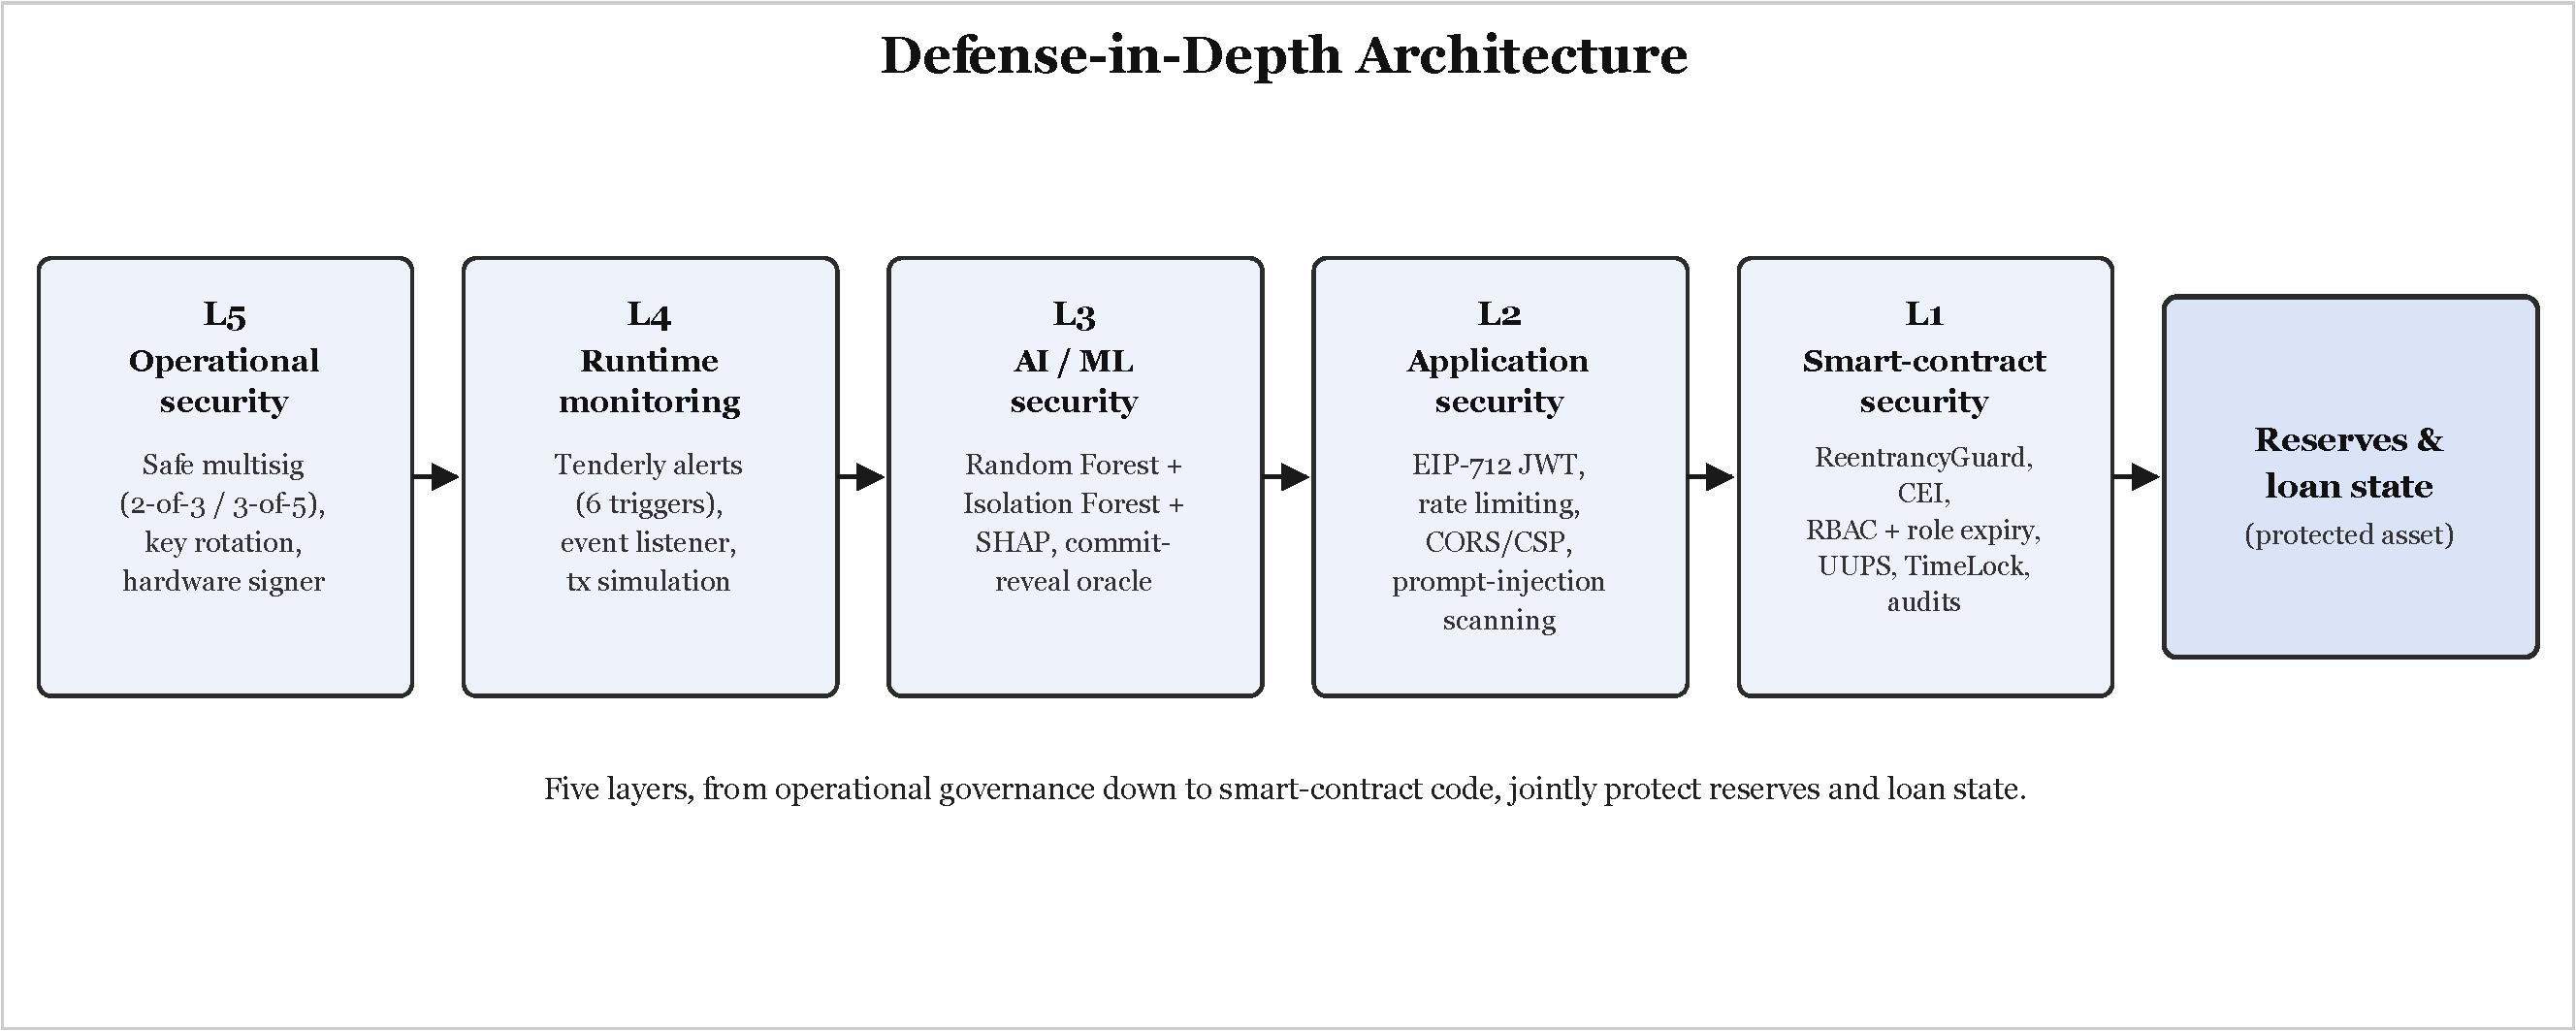
\includegraphics[width=0.78\textwidth,keepaspectratio]{fig-defense-in-depth_updated.pdf}
\caption{Five-layer defense-in-depth; human confirmation remains on the money path.}
\label{fig:defense}
\end{figure}

\begin{table}[H]
\centering
\footnotesize
\caption{Permission structure (network membership / access control).}
\label{tab:perms}
\begin{tabular}{@{}p{4.3cm}ccccc@{}}
\toprule
\tablehead Action & Client & LB Admin & NB Admin & WB Admin & Agent \\
\midrule
View own loan / public reserves & Y & Y & Y & Y & Read \\
Submit loan / pay installment & Y & N & N & N & Write$^*$ \\
\rowcolor{RowShade}
Approve / reject loan & N & Y & N & N & N \\
Freeze account / SAR & N & Y & Y & Y & N \\
\rowcolor{RowShade}
Set borrow rate & N & N & Y & Y & N \\
Change reserve ratio & N & N & N & Y & N \\
\rowcolor{RowShade}
Full audit log & N & Y & Y & Y & N \\
\bottomrule
\end{tabular}\\[2pt]
{\footnotesize $^*$Write tools require explicit human confirmation before the wallet signs.}
\end{table}

\begin{figure}[H]
\centering
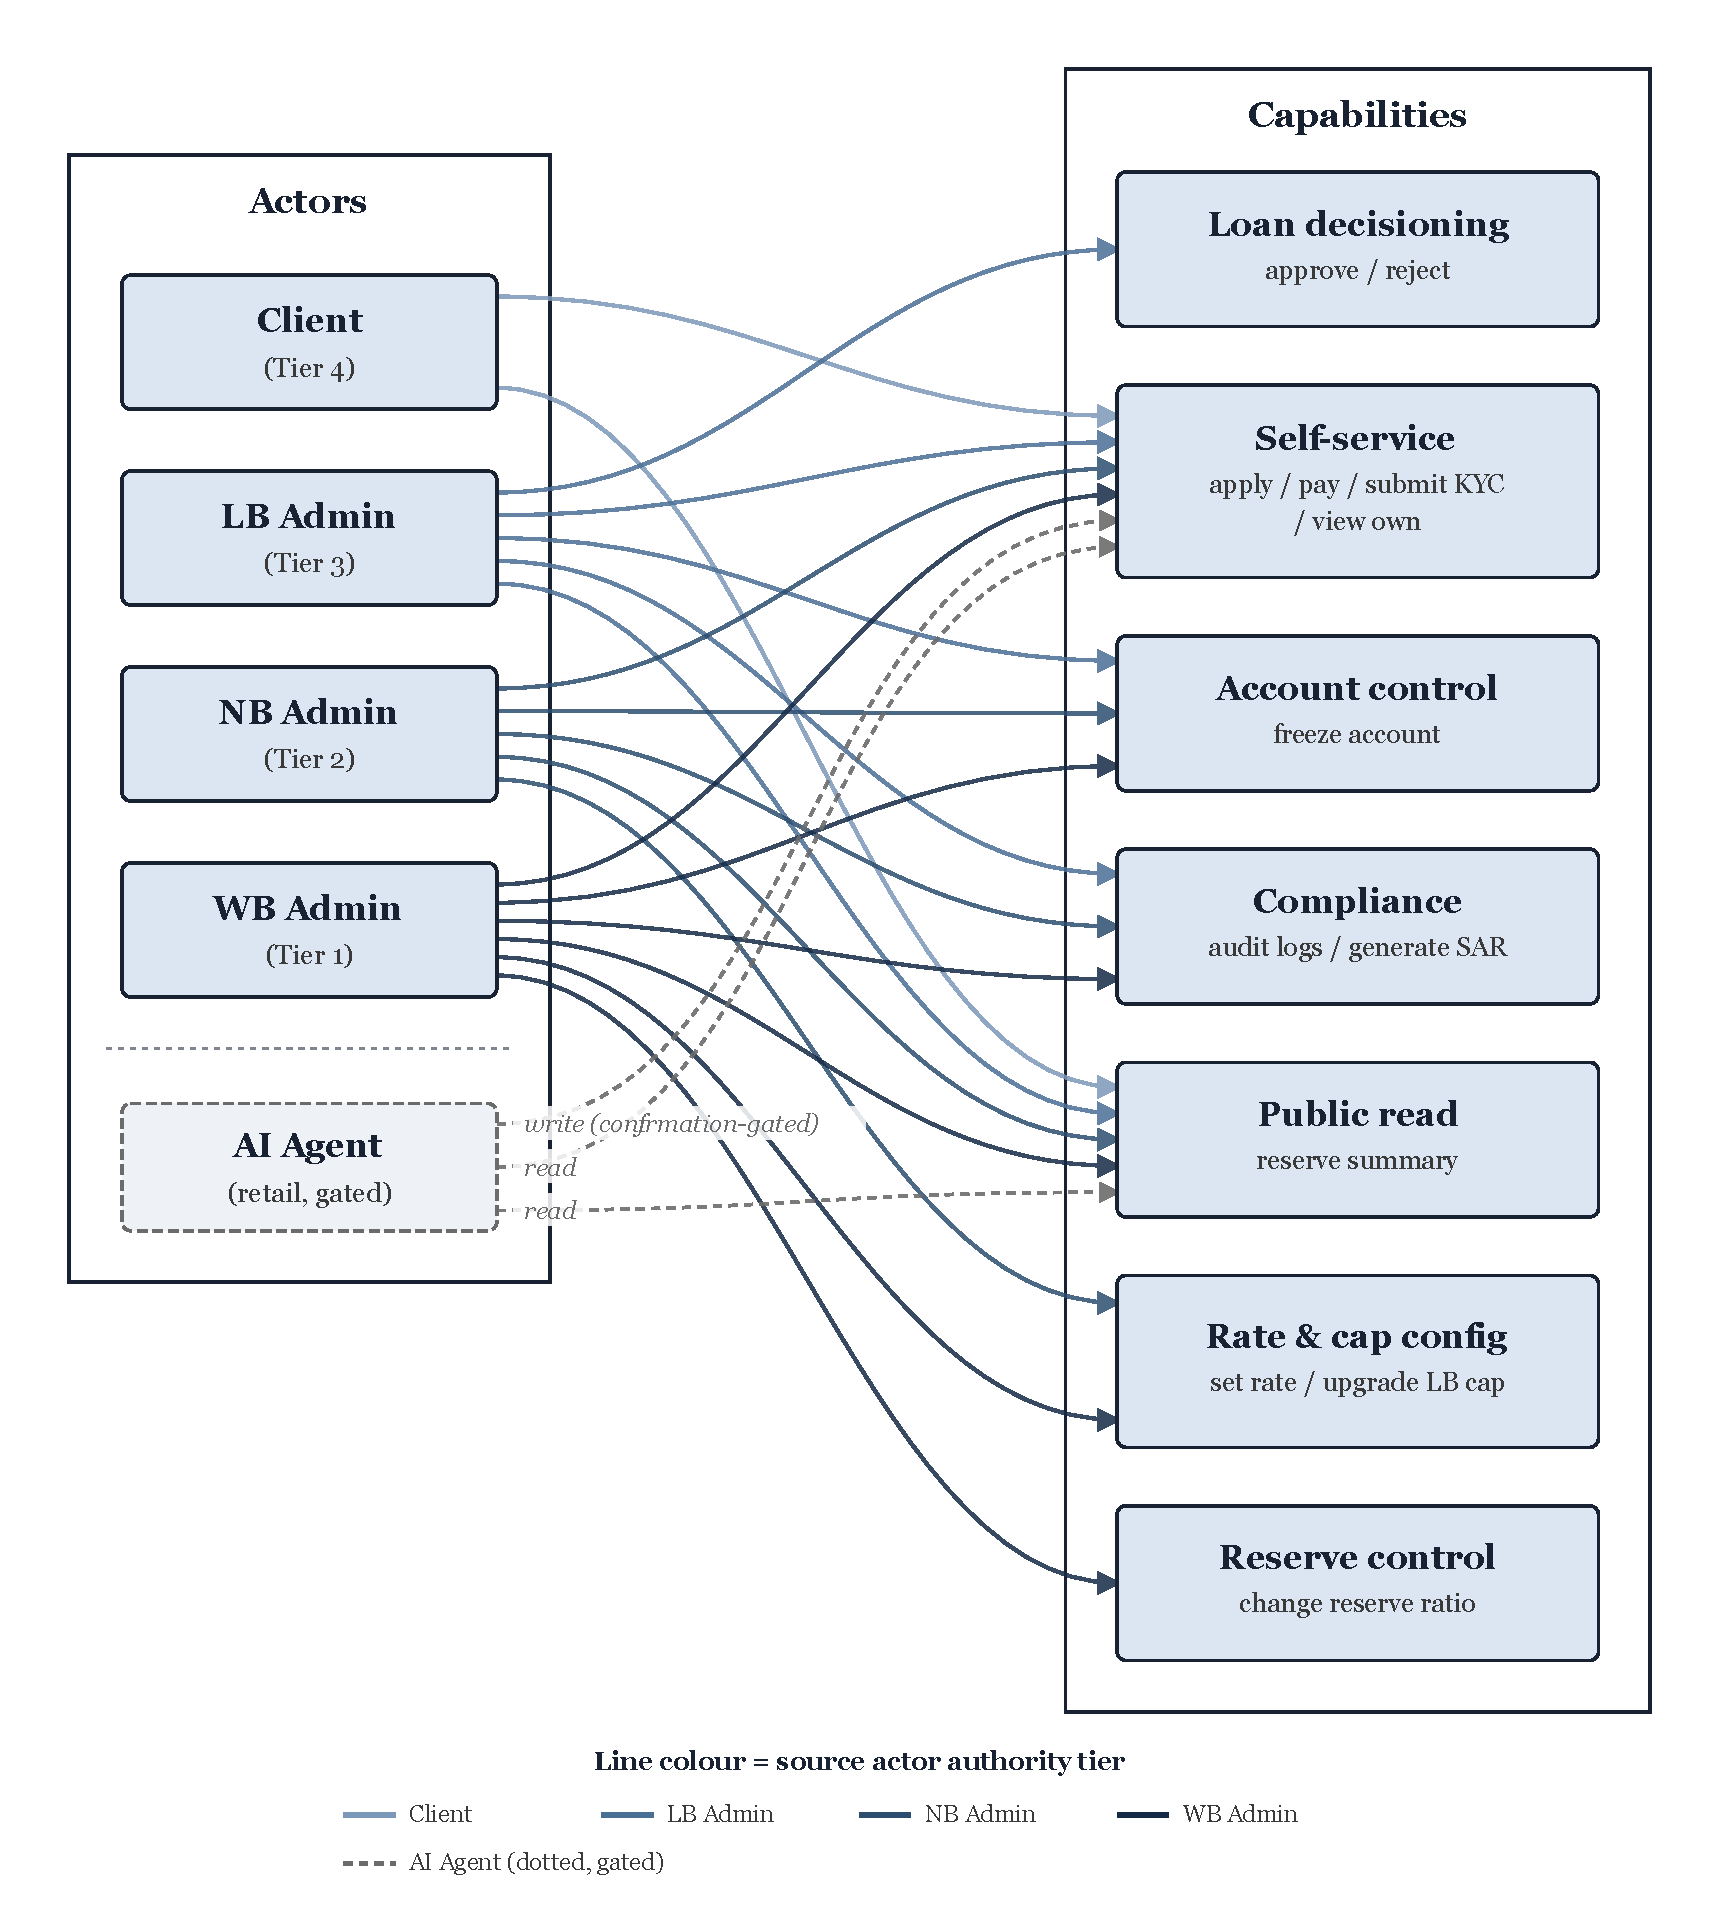
\includegraphics[width=0.55\textwidth,keepaspectratio]{Ch3_actor-permission-matrix_updated.pdf}
\caption{Actor--permission matrix used to derive contract modifiers and API RBAC.}
\label{fig:permfig}
\end{figure}

\subsection{Governance (checklist)}

Governance is split exactly as the evaluation scheme asks. Parameter changes use a 48-hour timelock controller and 60\% of the admin-role snapshot. Emergency pause requires two-thirds of the emergency Safe. Figure~\ref{fig:gov} shows the dual path: slow democratic change versus a fast circuit-breaker.

\begin{figure}[H]
\centering
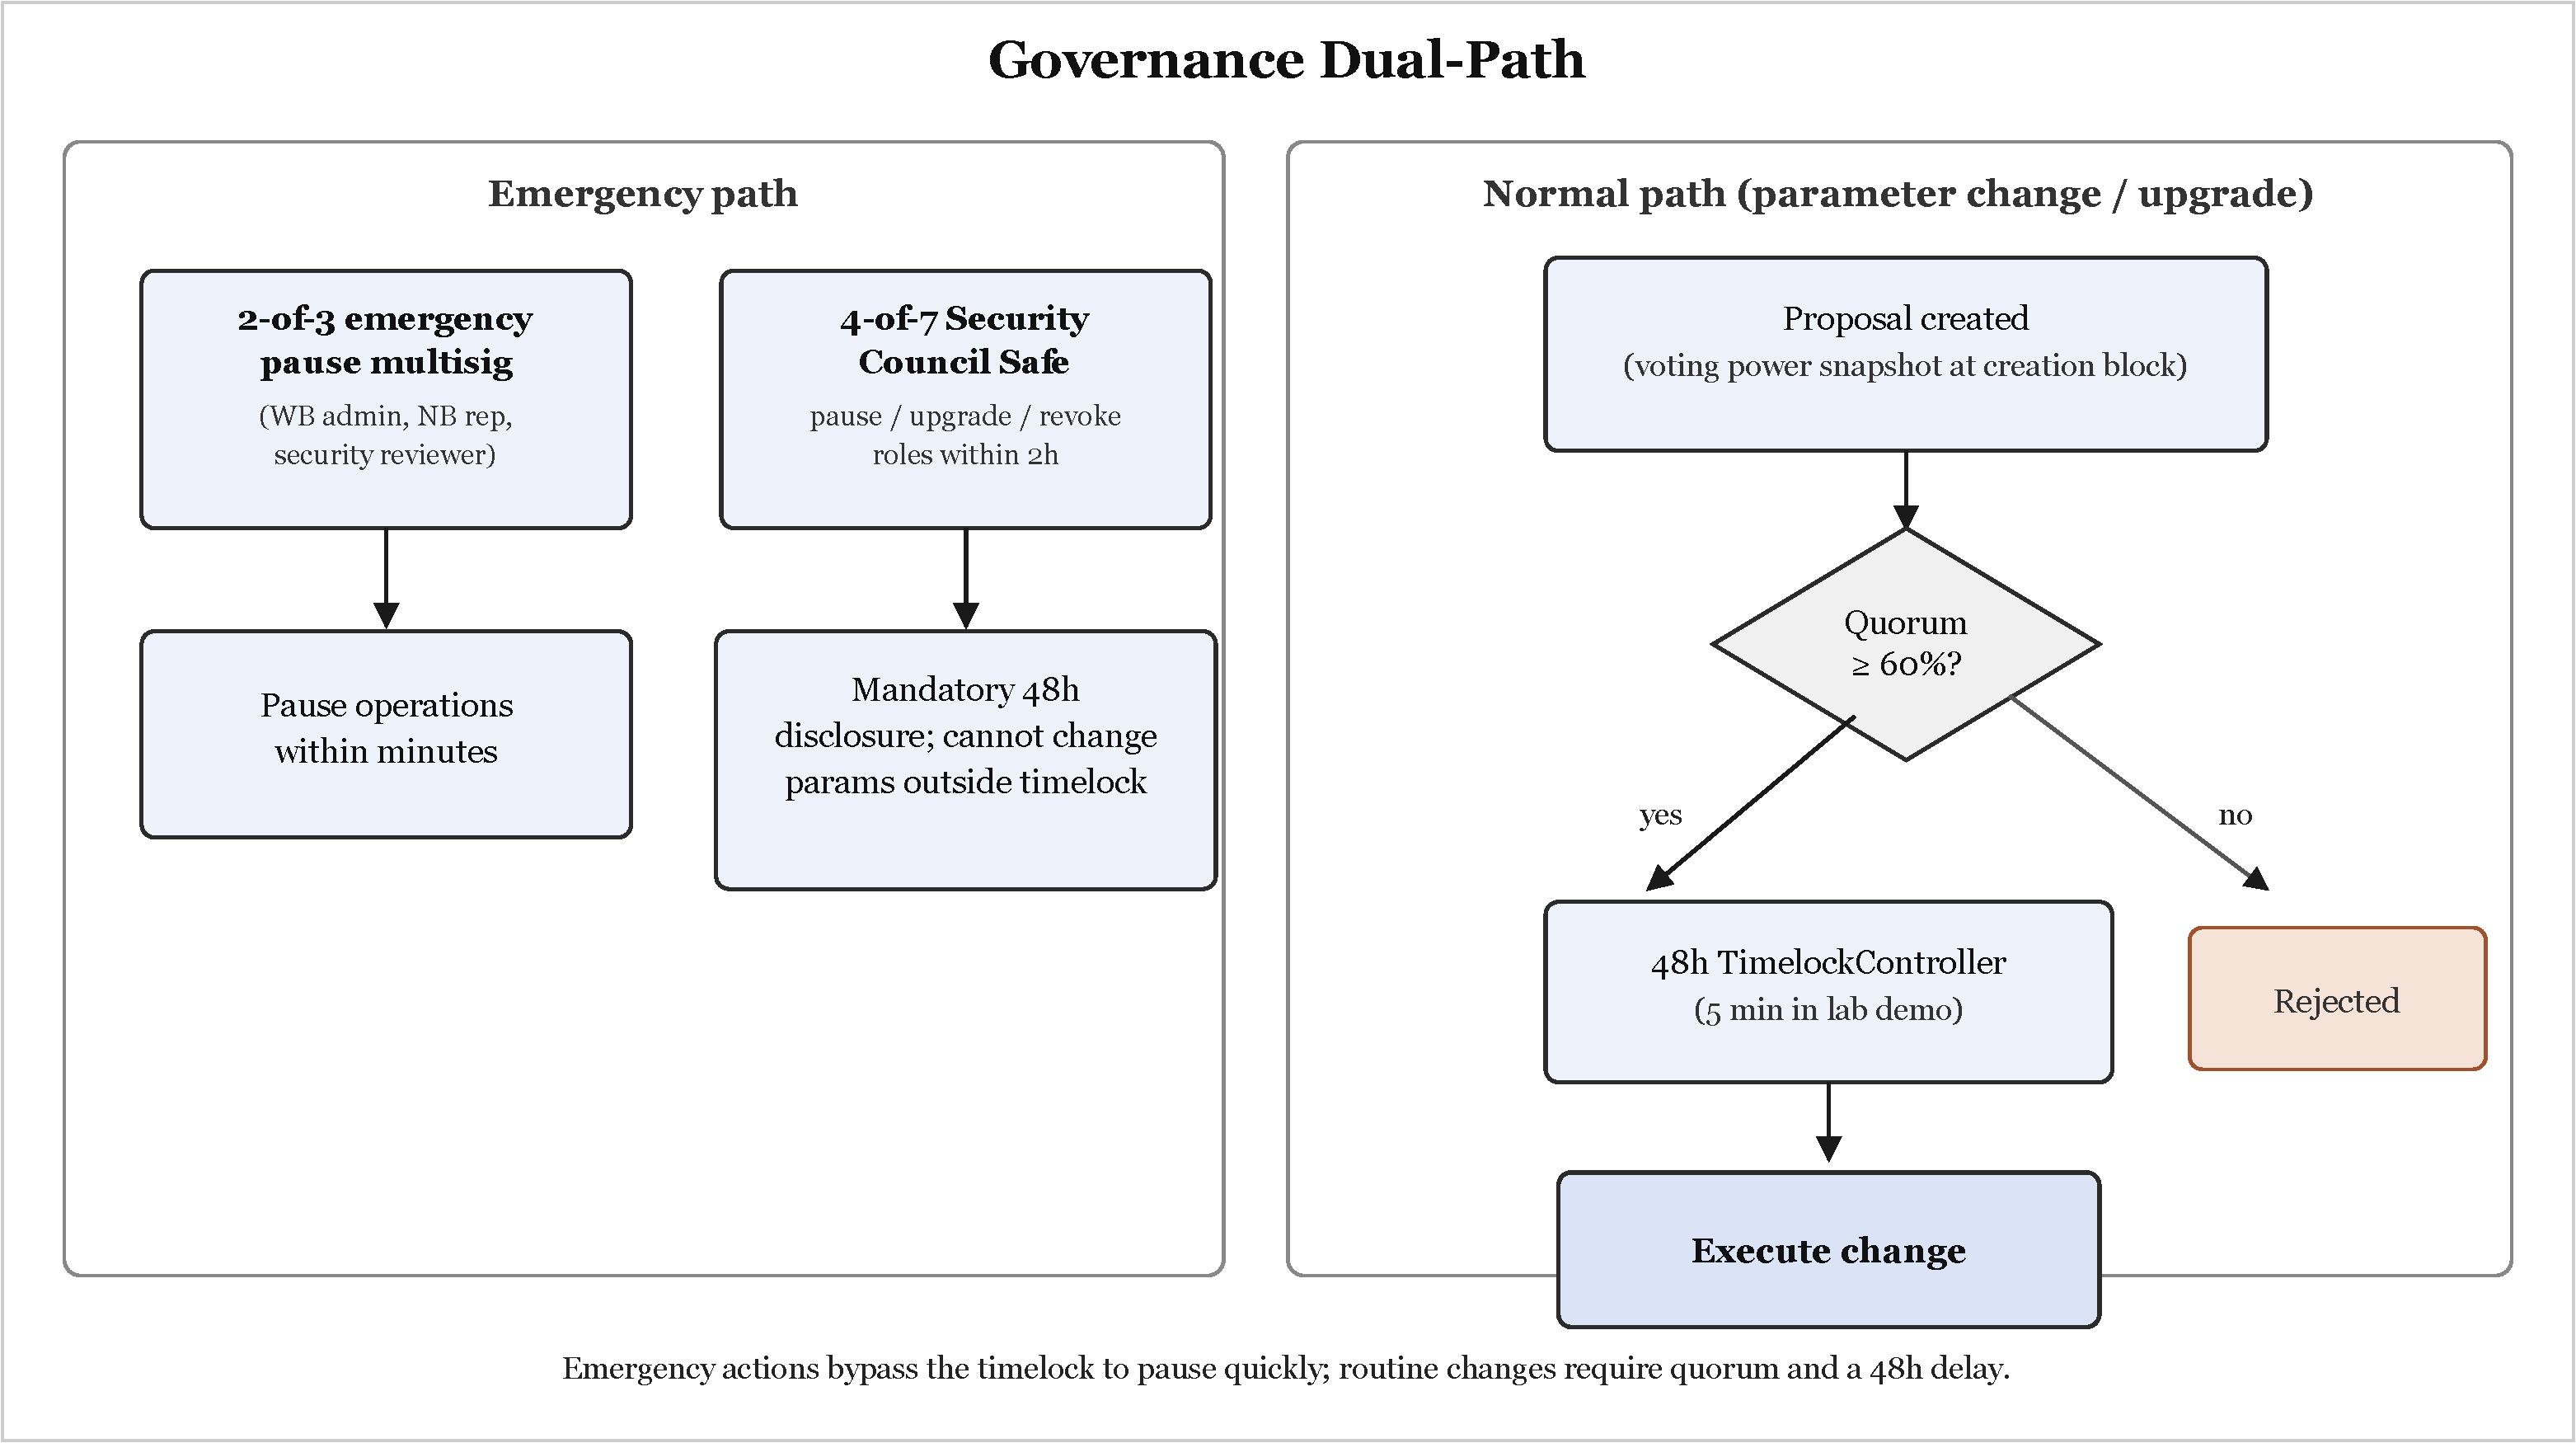
\includegraphics[width=0.84\textwidth,keepaspectratio]{fig-governance-dual-path_updated.pdf}
\caption{Dual-path governance: timelocked upgrades versus emergency pause.}
\label{fig:gov}
\end{figure}

\paragraph{Network membership governance.}
\begin{itemize}
  \item \textbf{On-boarding.} World Bank Admin registers a National Bank (institutional KYC off-chain, role on-chain). National Bank registers Local Banks. Local Bank onboards clients after Level~1 KYC (government ID + selfie stored off-chain; hash on record). Group clients add group verification.
  \item \textbf{Off-boarding.} Roles revoked on-chain; open loans still settle under the contract; freeze is available for SAR. Retail off-boarding does not burn repayment history on the SBT (reputation remains, access can be paused).
  \item \textbf{Regulatory oversight.} A Regulatory Authority actor has read-only audit packaging; cannot allocate capital. Sandbox reporting is an off-chain SLA on top of public events.
  \item \textbf{Permission structure.} Hierarchical RBAC (Table~\ref{tab:perms}); World Bank Admin via Safe, not a hot wallet.
  \item \textbf{Network operations.} Public PoS validators operate the chain; CWB operators run API, listener, ML, and Safe signers. Pause registry is per-function so a lending pause need not halt reserve views.
\end{itemize}

\paragraph{Business network governance.}
\begin{itemize}
  \item \textbf{Charter and operations.} Mandate: transparent hierarchical development credit. Products: downward allocation, retail lifecycle, group lending, savings, interbank and upward facilities. Charter parameters (reserve ratio, kink, bonuses) live in contracts behind timelock.
  \item \textbf{Common services.} Shared Credit Passport, insurance fund, event schema, and (production) price/PoR oracles. Banks do not run private copies of the score board.
  \item \textbf{SLA and regulatory compliance.} Testnet: best-effort. Sandbox: documented recovery RPO/RTO, SAR workflow (anomaly $\to$ freeze $\to$ compliance queue, Figure~\ref{fig:sar}), hash-only PII, explainable-AI artifacts for officers. No claim of a banking licence in this paper.
\end{itemize}

\paragraph{Technology infrastructure governance.}
\begin{itemize}
  \item \textbf{Distributed IT.} Consensus is public; CWB servers are replaceable because balances are not in them. Anyone may verify with a node and the contract addresses.
  \item \textbf{Technology assessment.} EVM+Solidity selected over Fabric/Corda/Solana as above; zkEVM is the production bias; Sepolia/Amoy are the stability bias for the prototype.
  \item \textbf{On-chain / off-chain services.} Section above; event listener is the only legal writer of projection tables for credit/loan mirrors.
  \item \textbf{Risk mitigation.} Tables~\ref{tab:bizrisk}--\ref{tab:techrisk}; Slither+Mythril and Foundry fuzz in the verification phase; 300-wallet simulation planned for gas and reserve dynamics.
\end{itemize}

\begin{figure}[H]
\centering
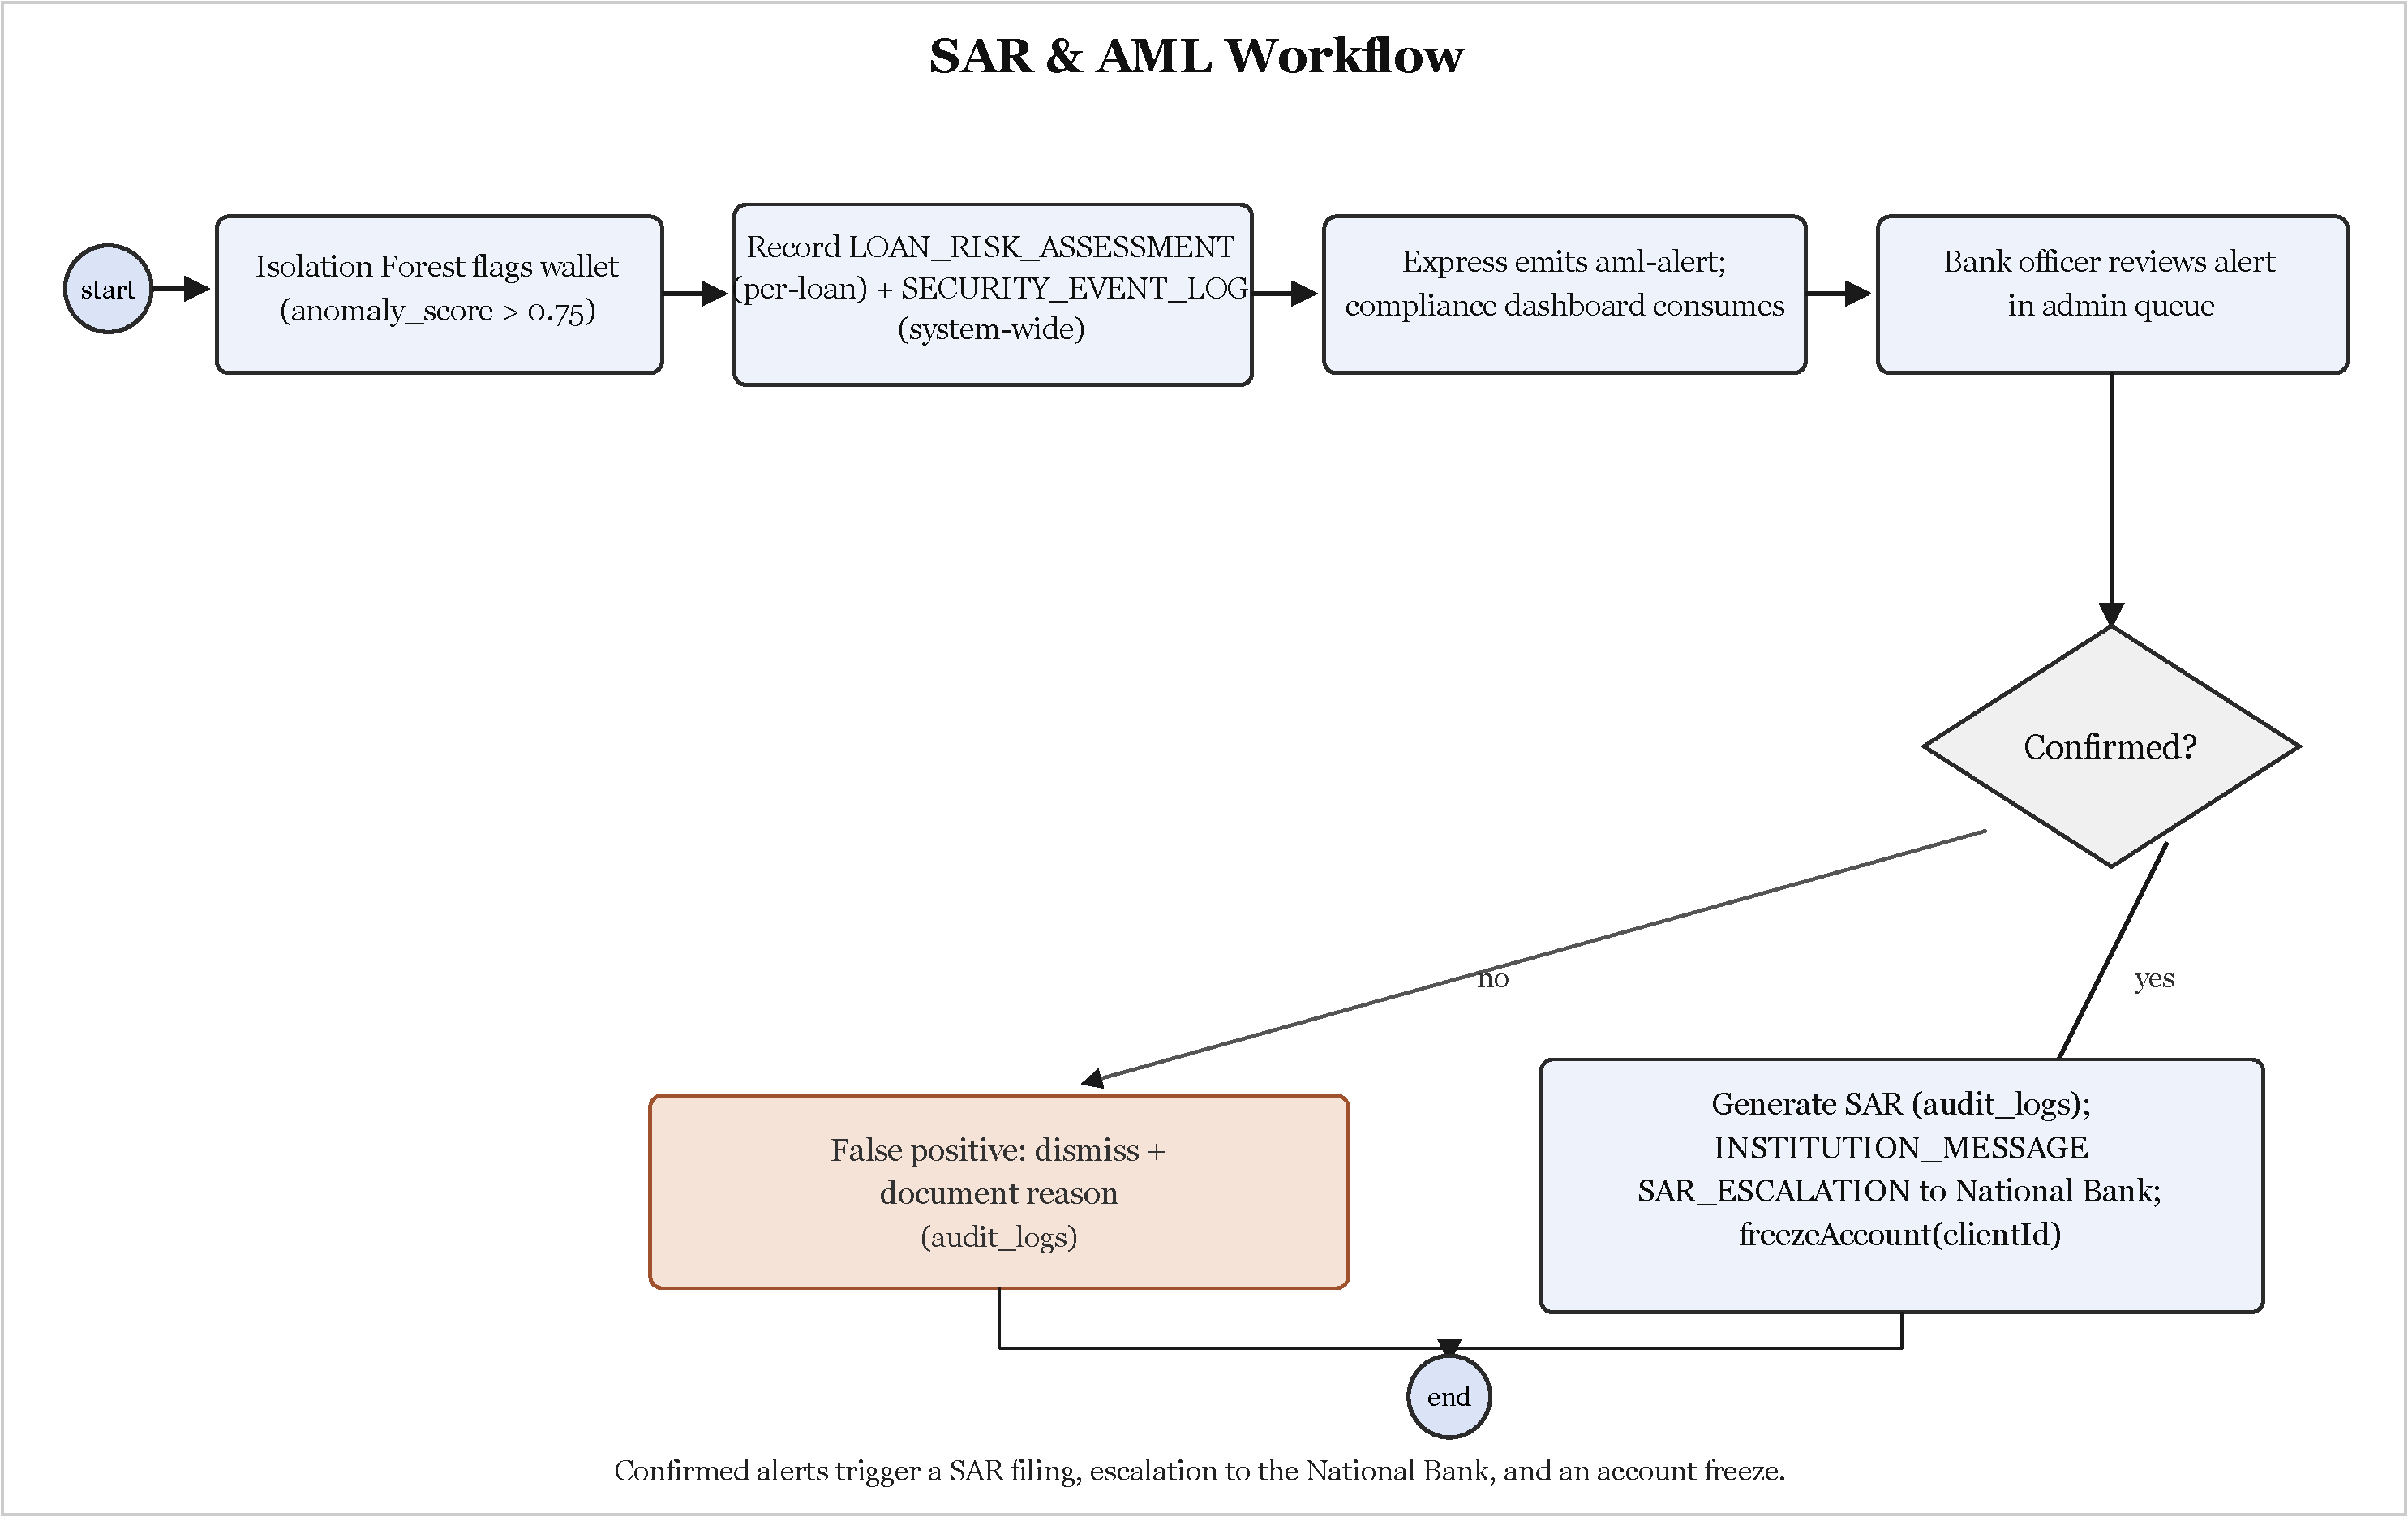
\includegraphics[width=0.80\textwidth,keepaspectratio]{fig-sar-aml-workflow_updated.pdf}
\caption{SAR / AML path: anomaly flag, freeze, and human compliance review.}
\label{fig:sar}
\end{figure}

\subsection{Prototype evidence (front-end + chain write)}

The repository already contains compilable \texttt{WorldBankReserve} / \texttt{NationalBank} / \texttt{LocalBank} contracts, 42 Hardhat tests, Express loan/bank/auth routes, a React+Wagmi wallet shell, a FastAPI \texttt{/score} scaffold, and Sepolia/Amoy deploy scripts. That satisfies the spirit of the prototype rule (UI + blockchain writes) while the remaining lifecycle and oracle wiring follow the 16-week four-phase plan (foundation $\to$ lending UX $\to$ ML/agent $\to$ verification).

%----------------------------------------------------------------------
\section{Revenue and Distribution}
\label{sec:revenue}
% 10 points
%----------------------------------------------------------------------

\subsection{How value is generated (not only cash)}

Revenue in the BCOLBD sense is \textit{value}, which may be money. CWB produces both.

\textbf{Monetary.}
\begin{itemize}
  \item Interest split on active loans: depositor yield + InsuranceFund (5\%) + protocol spread (NIM on hierarchical on-lending).
  \item Interbank pool spread, strictly interior to the downward curve so the protocol is paid for matching, not for trapping liquidity.
  \item Disclosed FX / treasury spread when \texttt{FXModule} / \texttt{TreasurySwap} are enabled.
  \item Optional sandbox SaaS to a development bank (support, dashboards)---secondary, not required for the protocol to clear.
\end{itemize}
There is \textbf{no ICO and no governance-token pump} in this design. Capture is spread on real credit and payments.

\textbf{Non-monetary (often larger for public partners).}
\begin{itemize}
  \item Lower-tier visibility into parent reserves (trust that today costs audits and correspondent float).
  \item Portable Credit Passport that cuts repeat origination cost.
  \item Regulator-ready event history for supervised credit.
  \item Inclusion: group products for clients who cannot post crypto collateral.
\end{itemize}

\textbf{Unit economics (planning, not audited forecast).} A full retail lifecycle is 27--32 on-chain steps. At L2/testnet prices this is about \$0.011 vs.\ \$2.40--\$4.80 on L1---immaterial against interest on a \$25{,}000 ticket at 8\% APR. Prototype build cost is \$0 (public testnets, open-source toolchain, local/Colab ML). Three-year planning case at 10\% discount: benefits \$48k / \$72k / \$96k against costs \$6k / \$8k / \$10k after \$6k setup $\Rightarrow$ NPV $\approx$ \$150k, accounting ROI $\approx$ 620\%, break-even on the order of 200--300 active loans once an 8\% default and \$500/month infra assumption are included. These numbers size the SOM; they are not a fund-raise deck.

\subsection{Go-to-market and next steps}

\begin{enumerate}
  \item \textbf{Now (competition).} Open-source testnet DApp: UI, contracts, ML baseline, this white paper, poster, and 10-minute pitch. Public repo is the distribution channel for reviewers.
  \item \textbf{Sandbox (0--12 months).} One Local Bank innovation team; MockUSDC or authorised test stablecoin; capped Bronze/Silver tickets; supervisor read dashboard; MFS cash-in via existing agent network (off-chain fiat, on-chain claim).
  \item \textbf{National on-lending (12--24 months).} A development bank as Tier~2; live reserve ratio; Chainlink PoR; independent contract audit; insurance-fund policy with a regulated partner.
  \item \textbf{Corridor expansion (24--36 months).} Second jurisdiction only after single-chain operations are dull. Still no bridge; if two chains are ever required, native issuance plus attested burn/mint under legal contract---not a third-party lock.
\end{enumerate}

Distribution to end clients is through \textbf{the Local Bank they already know}, not through a crypto exchange. Officers keep the yes/no. The chain keeps them honest about reserves, roles, and history. That is the launch plan: encode the institution, do not ask the institution to dissolve.

%----------------------------------------------------------------------
\section*{References}
\addcontentsline{toc}{section}{References}
\small
\setstretch{0.95}
\begin{enumerate}[label={[\arabic*]},leftmargin=1.6em,itemsep=0.2em]
\item \label{werner2022} S.~M. Werner et al., ``SoK: Decentralized Finance (DeFi),'' arXiv:2101.08778, 2022.
\item \label{defillama} DefiLlama, ``Lending protocols --- TVL and rankings,'' 2024--2026.
\item \label{aavev3} DefiLlama, ``Aave V3 TVL,'' 2026.
\item \label{maple} Fensory, ``Maple Finance --- institutional DeFi lending,'' 2026.
\item \label{findex} World Bank, \textit{The Global Findex Database 2021}.
\item \label{ifc2017} IFC, ``MSME Finance Gap,'' World Bank, 2017.
\item \label{cpmi147} CPMI/BIS, ``Correspondent Banking,'' 2016.
\item \label{fsb2020} FSB, ``Enhancing Cross-border Payments: Stage 3 Roadmap,'' 2020.
\item \label{wbremit} World Bank, ``Remittance Prices Worldwide,'' 2024.
\item World Bank, ``World Bank Group Tracks Project Funds with New Blockchain Tool,'' 2025.
\item JPMorgan, ``Kinexys Digital Payments,'' 2025.
\item \label{tan2023} B.~W. Tan, ``Central Bank Digital Currency and Financial Inclusion,'' IMF WP/23/69, 2023.
\item G.~Palaiokrassas et al., ``Leveraging Machine Learning for Multichain DeFi Fraud Detection,'' IEEE ICBC, 2024.
\item I.~T. Adom et al., ``LIME and SHAP in Loan Approval Systems,'' IJIEEB, 2025.
\item F.~T. Liu et al., ``Isolation Forest,'' IEEE ICDM, 2008.
\item \label{wang2021} B.~Wang et al., ``iBatch'' transaction batching, 2021.
\item York University BCCC, ``BCCC-DeFiFraudTrans-2025'' dataset.
\item V.~Buterin et al., soulbound tokens (decentralised society), 2022.
\item BIS Innovation Hub, ``Project Pine'' hierarchical reserve prototypes, 2025.
\item BCOLBD, \textit{Guideline \& Evaluation Scheme for Blockchain Category}, 2026.
\end{enumerate}

\vspace{2.2mm}
{\footnotesize\color{CoverNavy}\noindent\textit{End of white paper.} Page count includes cover, figures, tables, and references. No annexes.}

\end{document}
